\documentclass{article}
\usepackage[english,polish]{babel}
\selectlanguage{polish}

\title{\huge  \Huge \textbf{MOZA Projekt} \\ \textbf{Wzmacniacz Kaskodowy 4 (wariant B)}}
\date{\today}
\author{ \LARGE Jakub Półtorak}

\usepackage{amsmath}
\usepackage{amsfonts}
\usepackage{graphicx}
\usepackage[T1]{fontenc}
\usepackage{pdflscape}
\usepackage{rotating}

\begin{document}
\maketitle
\pagenumbering{gobble}
\newpage
\pagenumbering{arabic}
\tableofcontents

\pagebreak

\begin{center}
	\title{ \huge \textbf{Etap 1}}
\end{center}


\section*{Opis problemu}
Zadanie polega na doborze wartości elementów wzmacniacza tak, aby uzyskać maksymalnie duży iloczyn
GBW. Na układ nałożono dodatkowe ograniczenia w postaci minimalnego wzmocnienia dla małych częstotliwości $k_{u0} > 20 dB$ ($10 \frac{V}{V}$ dla źródła AC o amplitudzie 1 V) oraz minimalnej częstotliwości
granicznej $f_g > 200 MHz$ (rozumianej jako częstotliwość spadku o 3 dB względem $k_{u0}$).
\section{Sformułowanie matematyczne zadania optymalizacji}

\subsection{Optymalizacja jednokryterialna}
Poszukiwane jest minimum funkcji celu:
\[ \min\limits_{\textbf{x}\in \mathbf{R}^+  } f(\textbf{x}) \]
p.o.
\[ g_{i}(\textbf{x}) \leq 0 \ \ \ \  i=1..n_g\]
gdzie:
\[ f(\textbf{x}) = -(k_{u0}\cdot f_g)\]
\(\textbf{x}\) - wektor zmiennych optymalizowanych: \\
\begin{center}
	$\textbf{x}$ =
	$\begin{bmatrix}
			REE1 & REE2 & RE & RC2 & RC3 & CEE & CG
		\end{bmatrix}$,
\end{center}
\(k_{u0}(\textbf{x})\) - wzmocnienie dla małych częstotliwości, rozumiane jako wzmocnienie dla częstotliwości 1 kHz.\\
\(f_{g}(\textbf{x})\) - częstotliwość graniczna, rozumiana jako częstotliwość, dla której wzmocnienie
spada o 3 dB względem $k_{u_{0}}(\textbf{x}) $.

Parametry $k_{u0}(\textbf{x})$ oraz $f_g(\textbf{x})$ obliczane są w Matlabie na podstawie surowych danych ($U^{AC}_{out}(x,f)$) zwracanych
przez symulator LTSpice.

Dodatkowo, w zadaniu pojawiają się ograniczenia nieliniowe związane z wymaganiami projektowymi:\\
\begin{itemize}
	\item \(g_1(\textbf{x}): -(\frac{k_{u0}(\textbf{x})}{k_{u_{min}}}-1) <  0\) \\ Warunek minimalnego wzmocnienia, $k_{umin}=20dB$
	\item \(g_2(\textbf{x}): -(\frac{{f_g}(\textbf{x})}{f_{g_{min}}}-1)<0\) \\ Warunek minimalnej częstotliwości granicznej, $f_{gmin}=200 MHz$. Częstotliwość graniczna $f_g$ obliczana jest jako częstotliwość,
dla której wzmocnienie spada o 3 dB względem $ku_0$.
	\item \(g_3(\textbf{x}): b(\textbf{x})-b_{max}<0\) \\ Ograniczenie podbicia charakterystyki, $b_{max}=1dB$. Podbicie $b(\textbf{x})$ rozumiane jest jako różnica między maksymalnym poziomem wzmocnienia a $k_{u0}$ ((czyli $max(k_{u}(\textbf{x}))-b_{max}$)).Podbicie jest obliczane w Matlabie.

\end{itemize}
\subsection{Optymalizacja wielokryterialna}
Poszukiwane jest minimum funkcji celu:
\[ \min\limits_{\textbf{x}\in \mathbf{R}^+  } [f_1(\textbf{x}), f_2(\textbf{x})] \]
p.o.
\[ g_{i}(\textbf{x}) \leq 0 \ \ \ \  i=1..n_g\]
gdzie:
\[ f_1(\textbf{x}) = -k_{u0}\] \[ f_2(\textbf{x}) = -f_g\]
\(\textbf{x}\) - wektor zmiennych optymalizowanych: \\
\begin{center}
	$\textbf{x}$ =
	$\begin{bmatrix}
			REE1 & REE2 & RE & RC2 & RC3 & CEE & CG
		\end{bmatrix}$,
\end{center}
\(k_{u0}(\textbf{x})\) - wzmocnienie dla małych częstotliwości, rozumiane jako wzmocnienie dla częstotliwości 1 kHz.\\
\(f_{g}(\textbf{x})\) - częstotliwość graniczna, rozumiana jako częstotliwość, dla której wzmocnienie
spada o 3 dB względem $k_{u_{0}}(\textbf{x}) $.

Parametry $k_{u0}(\textbf{x})$ oraz $f_g(\textbf{x})$ obliczane są w Matlabie na podstawie surowych danych ($U^{AC}_{out}(x,f)$) zwracanych
przez symulator LTSpice.

Dodatkowo, w zadaniu pojawiają się ograniczenia nieliniowe związane z wymaganiami projektowymi (identyczne jak dla optymalizacji jednokryterialnej):\\
\begin{itemize}
	\item \(g_1(\textbf{x}): -(\frac{k_{u0}(\textbf{x})}{k_{u_{min}}}-1) <  0\) \\ Warunek minimalnego wzmocnienia, $k_{umin}=20dB$
	\item \(g_2(\textbf{x}): -(\frac{{f_g}(\textbf{x})}{f_{g_{min}}}-1)<0\) \\ Warunek minimalnej częstotliwości granicznej, $f_{gmin}=200 MHz$. Częstotliwość graniczna $f_g$ obliczana jest jako częstotliwość,
dla której wzmocnienie spada o 3 dB względem $ku_0$.
	\item \(g_3(\textbf{x}): b(\textbf{x})-b_{max}<0\) \\ Ograniczenie podbicia charakterystyki, $b_{max}=1dB$. Podbicie $b(\textbf{x})$ rozumiane jest jako różnica między maksymalnym poziomem wzmocnienia a $k_{u0}$ ((czyli $max(k_{u}(\textbf{x}))-b_{max}$)).Podbicie jest obliczane w Matlabie.

\end{itemize}




\section{Wyznaczenie przybliżenia początkowego rozwiązania}
Zgodnie z poleceniem zmodyfikowano domyślne wartości elementów tak, aby uzyskać rozwiązanie spełniające warunek minimalnej częstotliwości granicznej i wzmocnienia.
Ostatecznie, po wybraniu wartości, wektor \textbf{x} wygląda następująco:
\begin{center}
	$\textbf{x}$ =
	$\begin{bmatrix}
			5\Omega & 15\Omega & 320\Omega & 220\Omega & 200\Omega & 45p & 50p
		\end{bmatrix}$,
\end{center}

Wyniki w punkcie początkowym można zobaczyć na poniższym wykresie:

\begin{figure}[h]
	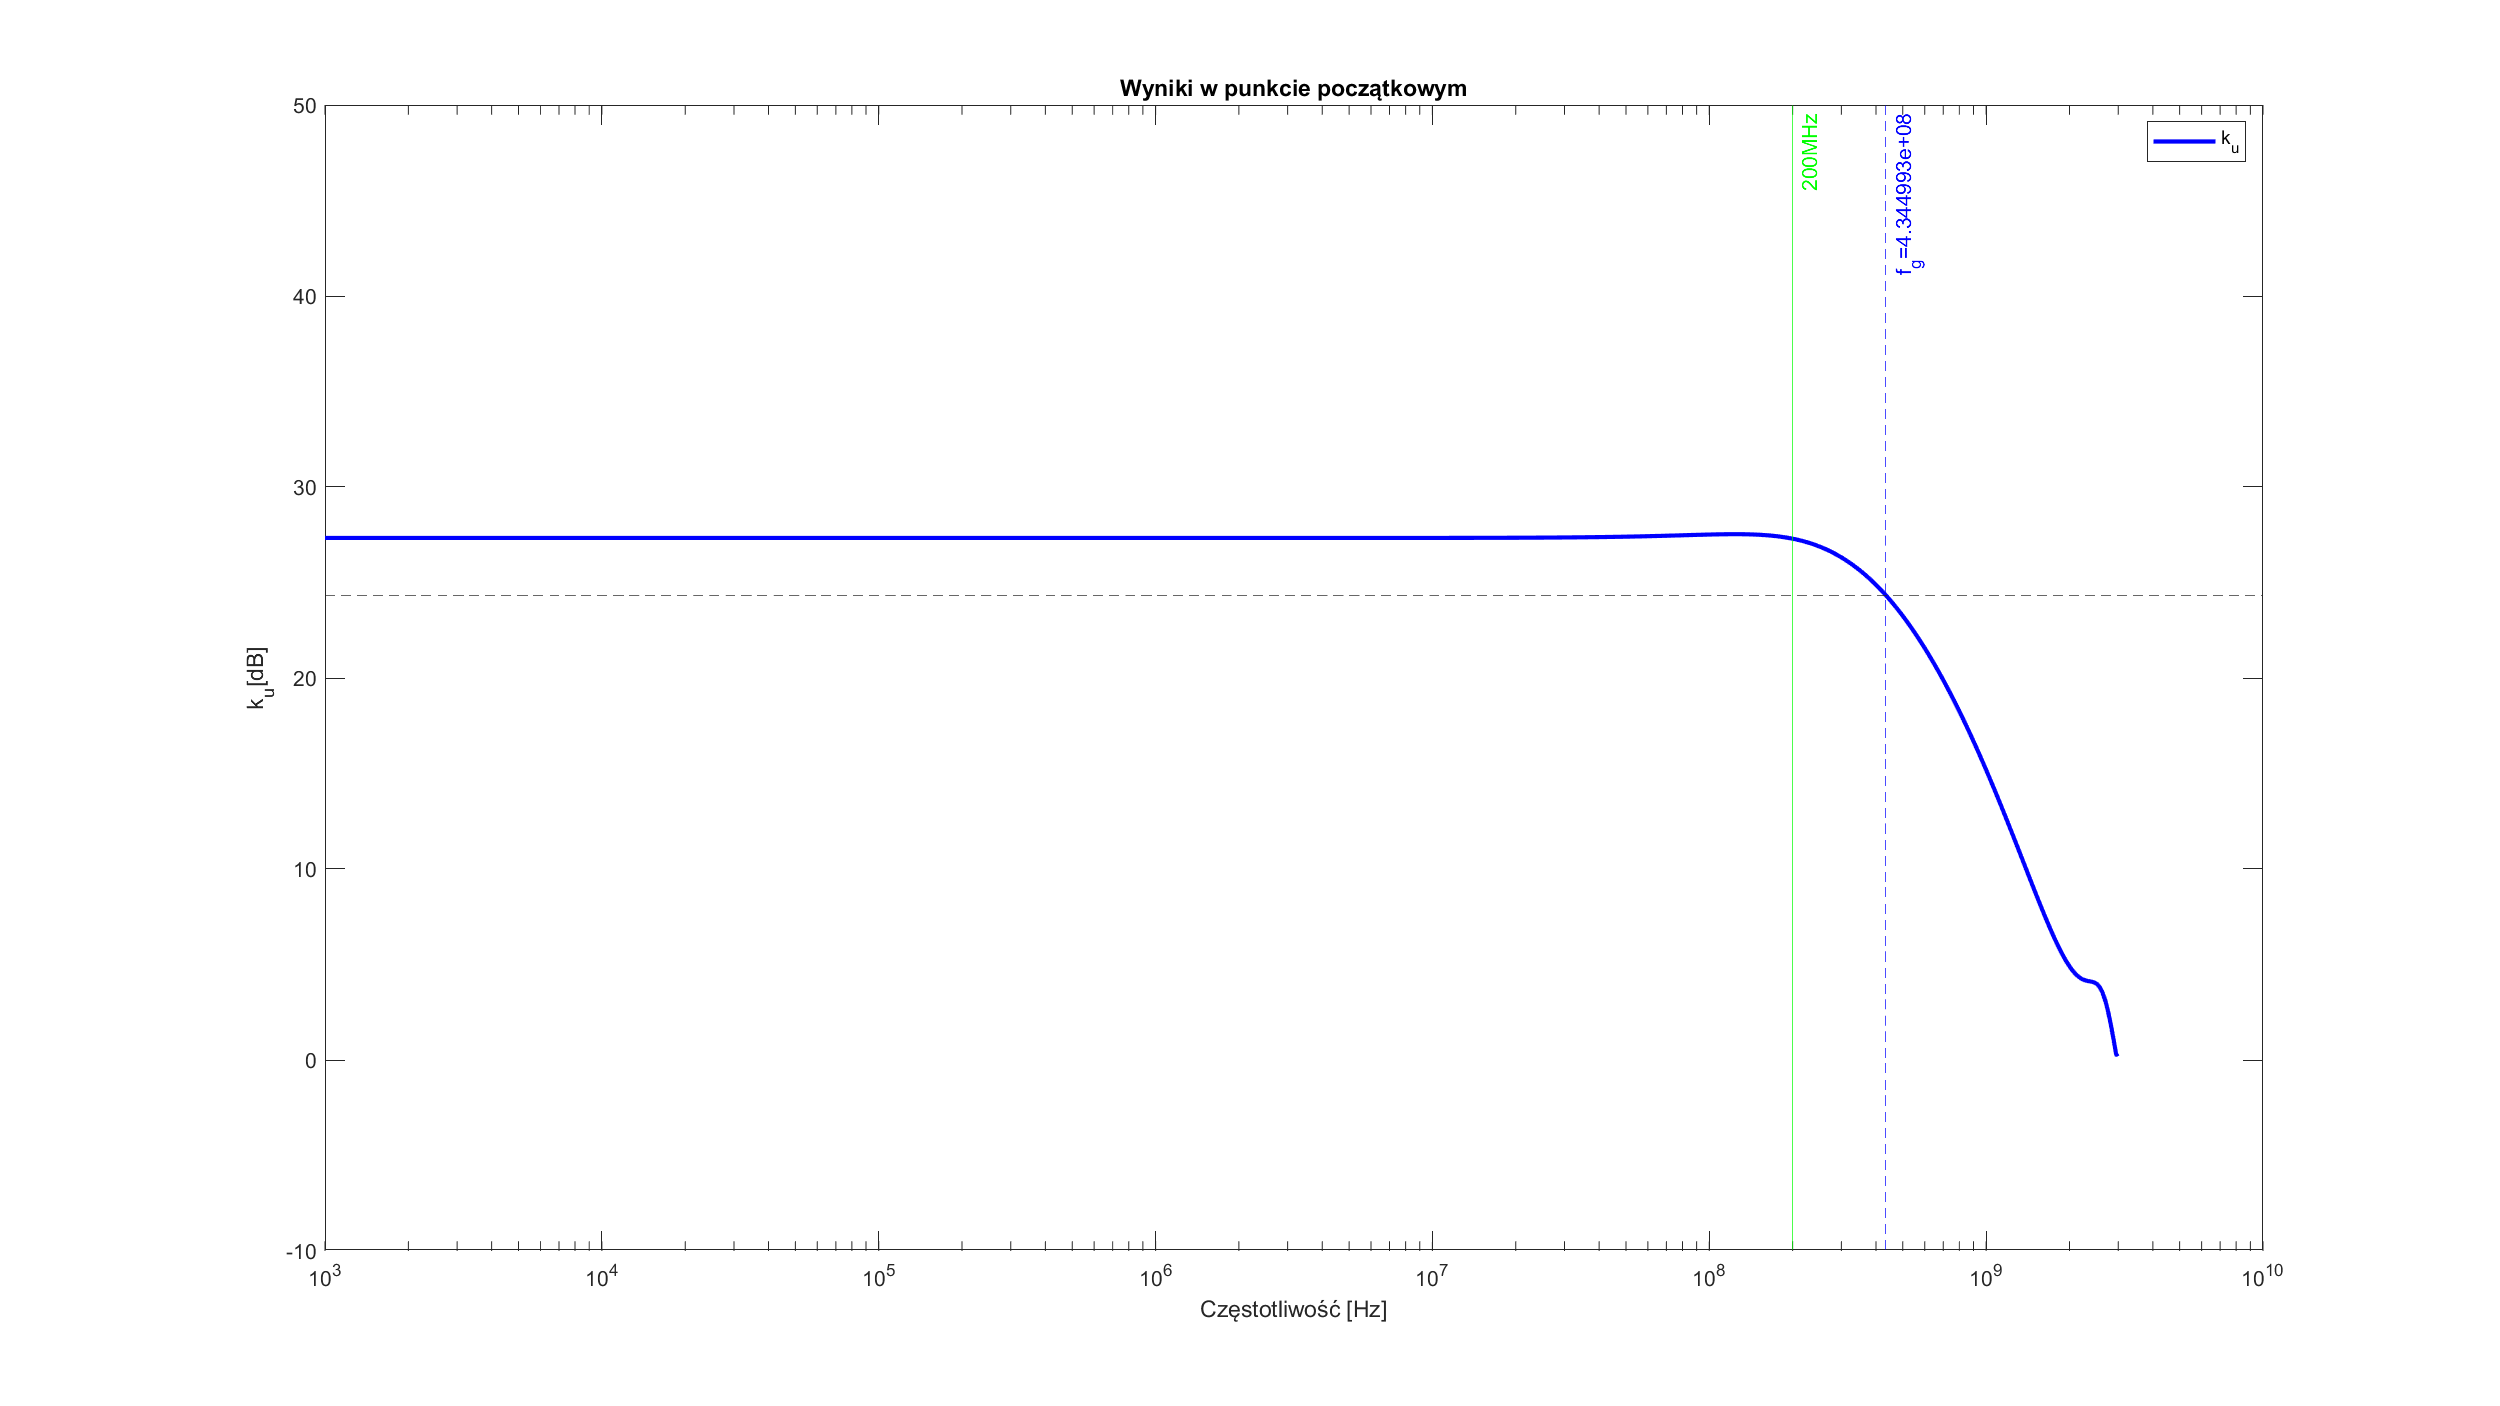
\includegraphics[width=12cm]{graphics/starting_point.png}
	\centering
	\caption{Charakterystyka układu w punkcie startowym.}
\end{figure}

Jak widać spełnione są warunki postawione w zadaniu (minimalna wartość wzmocnienia to 20 dB, przy źródle AC mającym 1 V amplitudy) oraz wzmacniacz pracuje prawidłowo (symulacja czasowa wykonan w LTSpice potwierdziła prawidłową pracę układu).
\pagebreak

Aby potwierdzić, że Matlab i Spice zwracają te same wyniki przeprowadzono symulację w LTSpice:
\begin{figure}[h]
	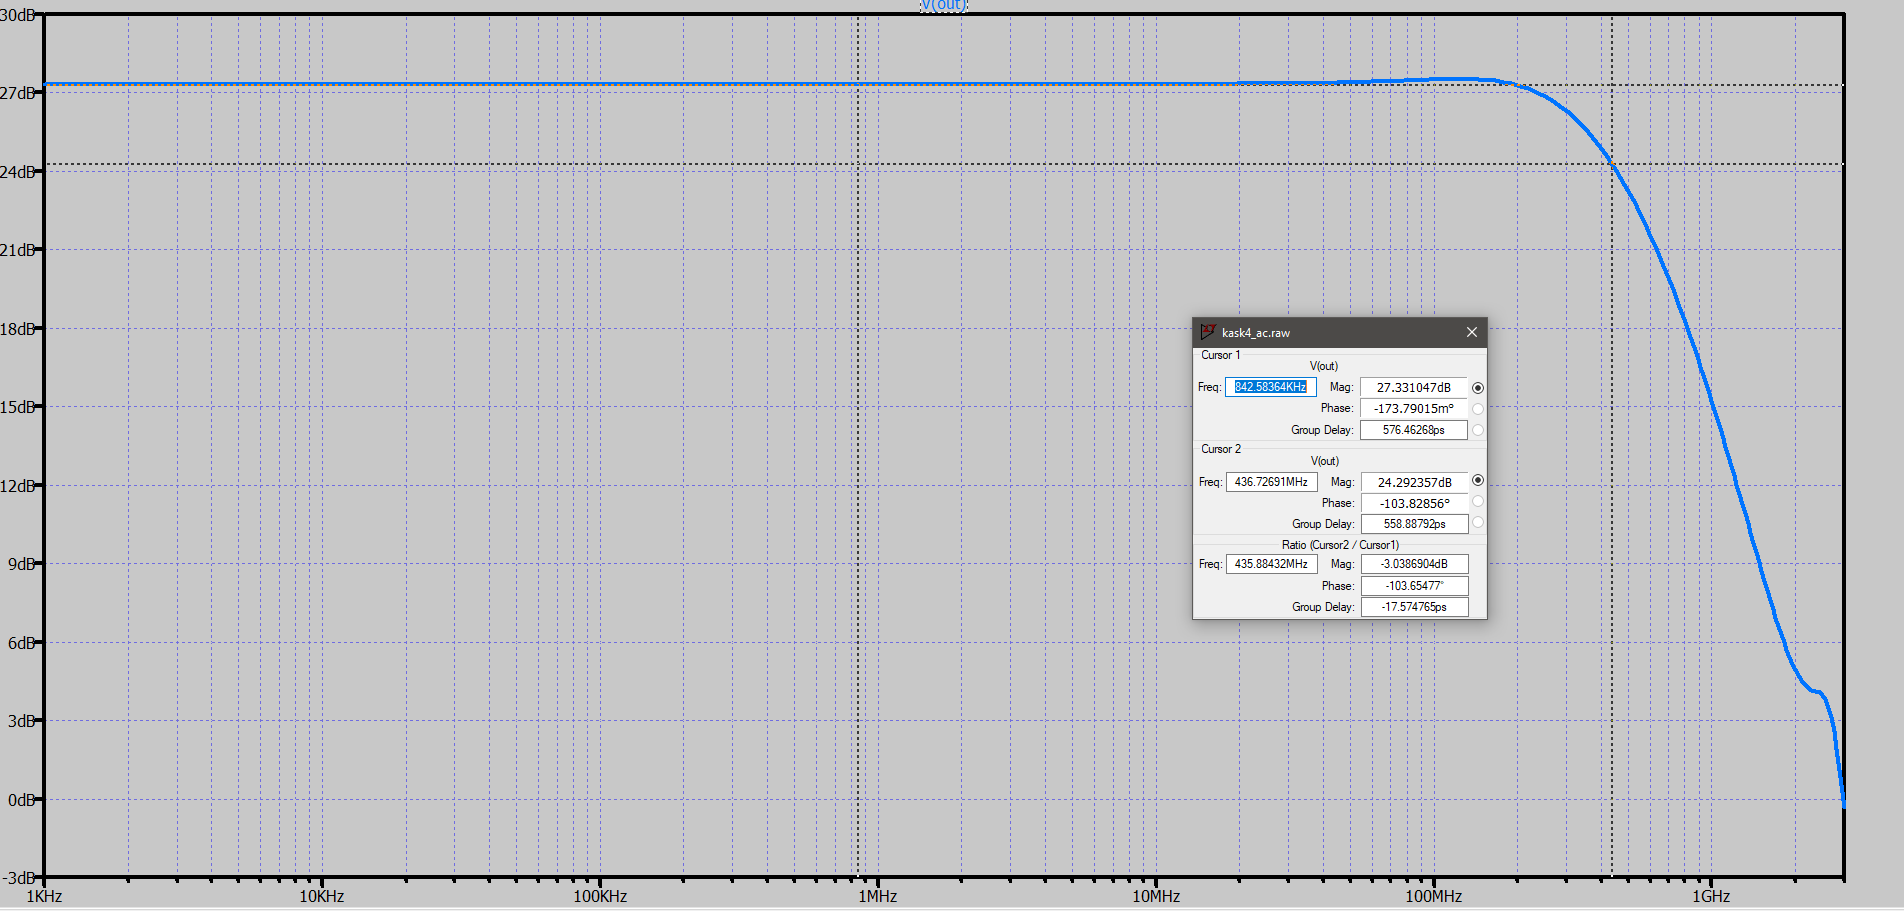
\includegraphics[width=12cm]{graphics/starting_point_spice.png}
	\centering
	\caption{Charakterystyka układu w punkcie startowym.}
\end{figure}




\section{Wyznaczanie parametrów roboczych, gładkość funkcji celu, opis kodu}
\subsection{Wyznaczanie parametrów roboczych}
W zadaniu badane są trzy parametry: częstotliwość graniczna, wzmocnienie oraz podbicie charakterystyki.

\subsubsection*{Podbicie $b$}
Podbicie rozumiane jest jako różnica między wzmocnieniem $k_{u0}$ a maksymalnym wzmocnieniem jakie osiąga charakterystyka ($max(k_{u}(\textbf{x}))-b_{max}$).
Maksimum charakterystyki jest wyznaczane przez interpolację (wielomian drugiego stopnia). Pozwala to dokładniej ustalić maksynmalne wzmocnienie i wygładza funkcję celu.
Efekty interpolacji widać na poniższym wykresie:
\begin{figure}[h]
	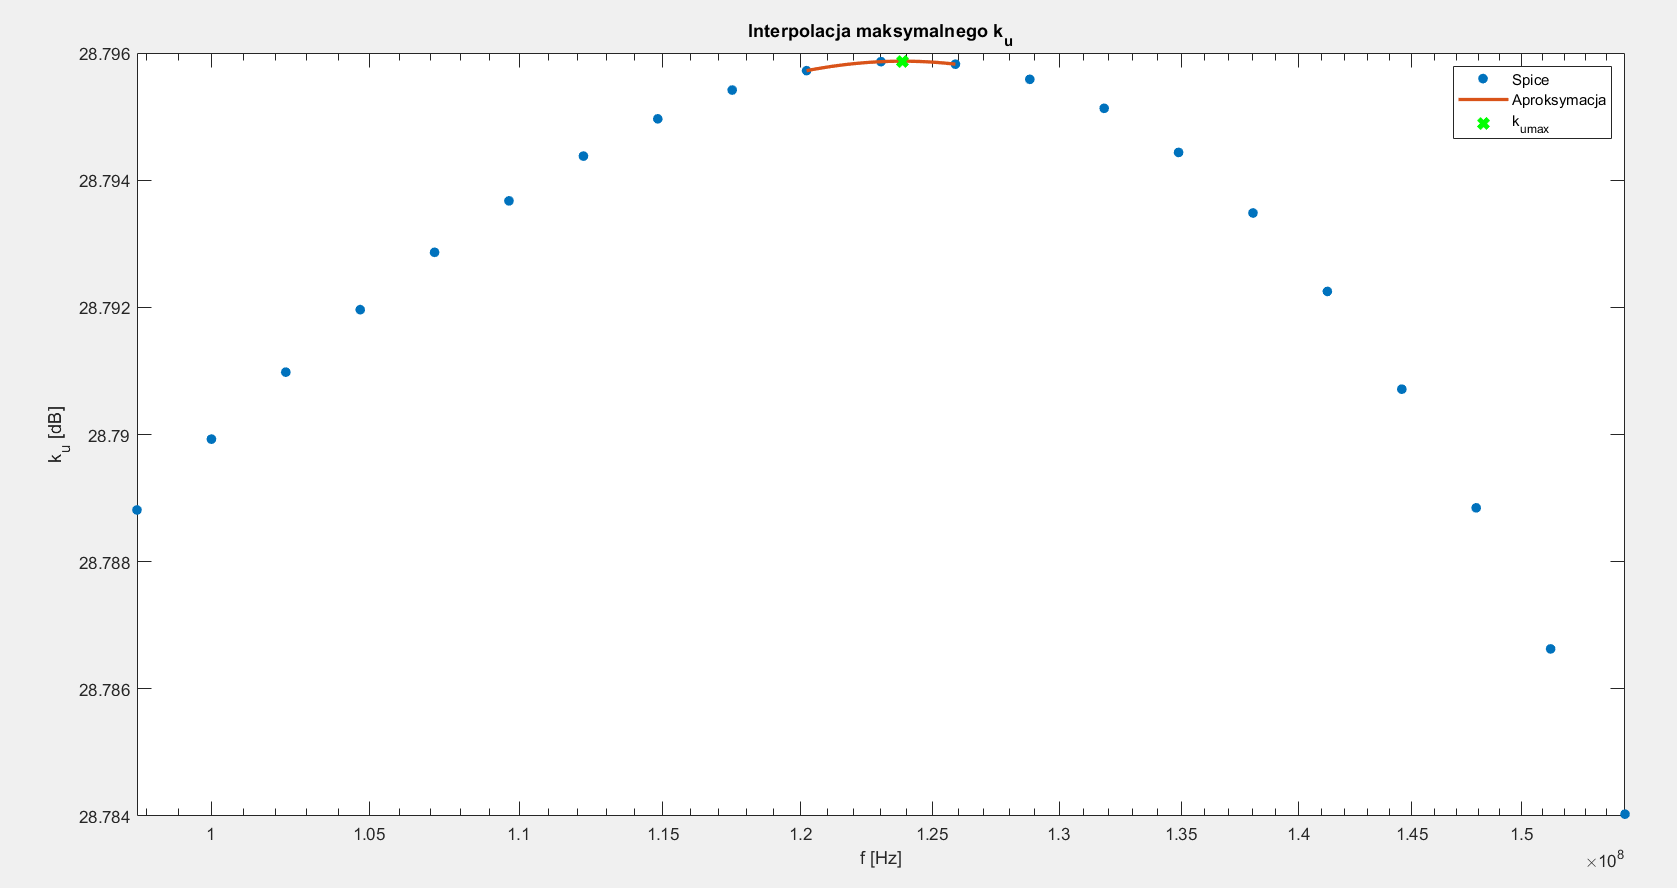
\includegraphics[width=8cm]{graphics/max_ku_interp.png}
	\centering
	\caption{Interpolacja maksimum charakterystyki.}
\end{figure}
\pagebreak
\subsubsection*{Wzmocnienie małoczęstotliwościowe $k_{u0}$}
Wzmocnienie $k_u$ rozumiane jest jako wartość wzmocnienia pozyskana z danych $U^{AC}_{out}(x,f)$ dla częstotliwości 1 KHz.

\subsubsection*{Częstotliwość graniczna $f_g$}
Częstotliwość graniczna wyznaczana jest jako częstotliwość, dla której wzmocnienie względem $k_{u{_0}}$ spada o 3 dB.
Ponieważ LTSpice zwraca wyniki w postaci punktów, uznano, że wymagana jest interpolacja częstotliwości granicznej. Interpolacja pozwoliła zminimalizować ''skoki'' w funkcji celu. Do interpolacji wykorzystano wielomian drugiego stopnia. Wynik interpolacji przedstawia poniższy wykres:
\begin{figure}[h]
	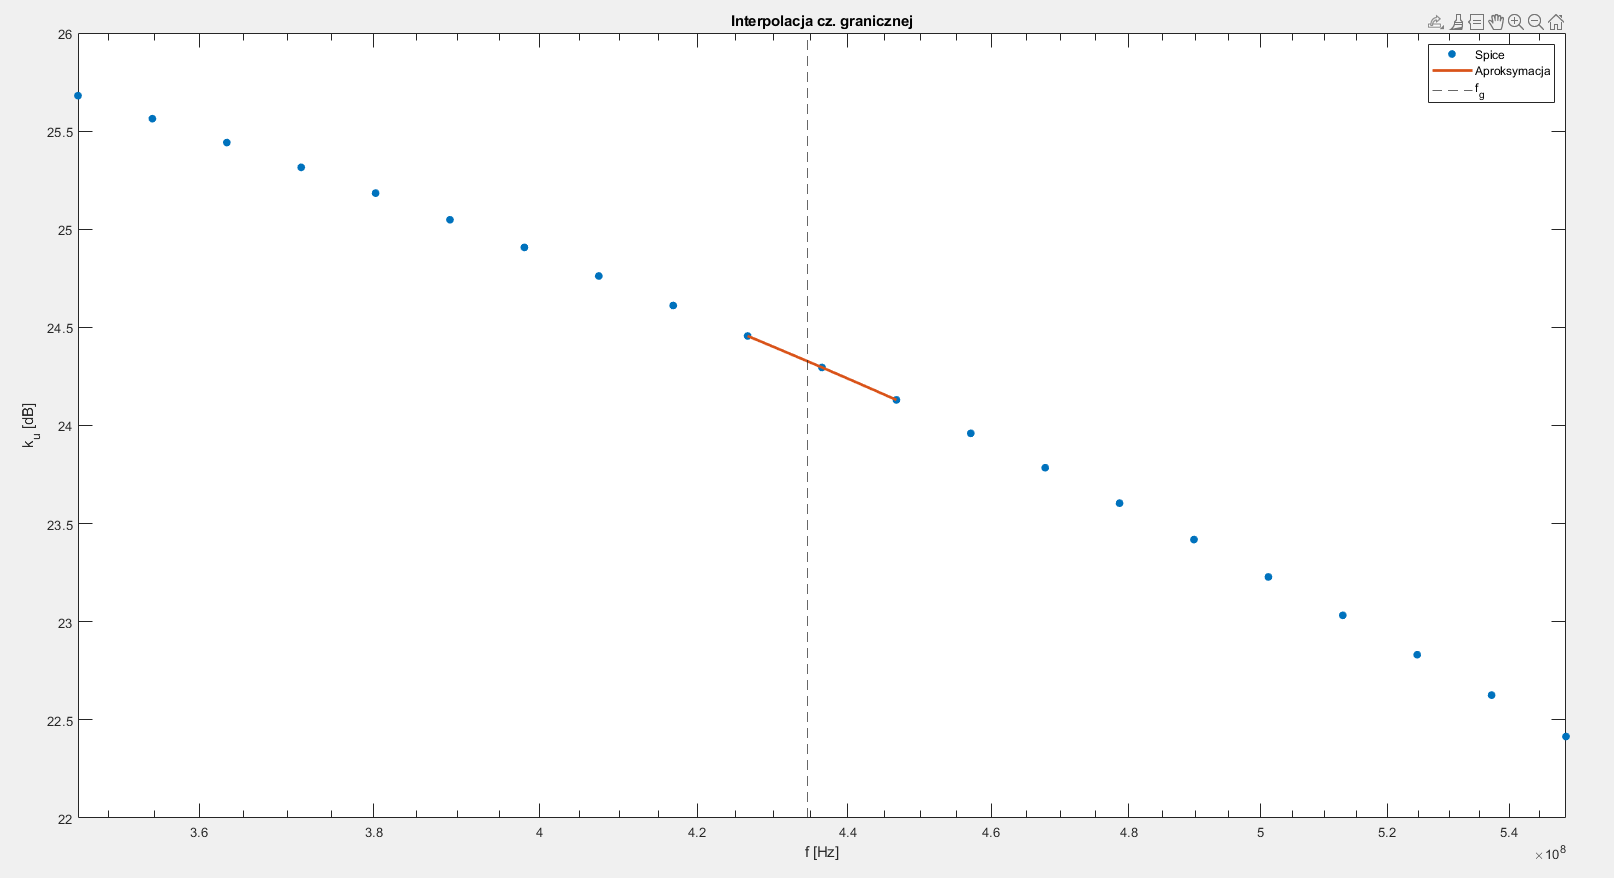
\includegraphics[width=8cm]{graphics/fg_interp.png}
	\centering
	\caption{Interpolacja częstotliwości granicznej.}
\end{figure}




\subsection{Gładkość funkcji celu i ograniczeń}
Przyjęto, że funkcja celu, w obrębie odpowiednich wartości elementów układu, jest ciągła. Tak długo, jak w układzie zmieniane są wartości pojemności i rezystancji i
nie powodują nieprawidłowej pracy układu zawsze możliwe będzie otrzymanie charakterystyki, która, nawet jeśli nie spełnia wymagań projektowych, daje ''sensowne'' wartości paremetrów roboczych (bez dużych skoków
np. wzrost wzmocnienia do 10000 dB).

Funckje ograniczeń i celu mogą być w niektórych przypadkach niegładkie. Może dojść do takiej sytuacji, gdy aktualny zestaw wartości elementów spowoduje powstanie charakterystyki,
dla której niektóre z parametrów roboczych nie są możliwe do obliczenia lub nie mają fizycznego sensu (np. płaska charakterystyka na poziomie 0 dB spowoduje, że nie istnieje częstotliwość graniczna rozumiana wg. zasad zdefiniowanych
na początku raportu, funkcja obliczająca zwraca wtedy 0). Punkty przejścia między ""dobrą"" a ""złą"" charakterystyką są właściwie punktami, gdzie funkcja nie jest gładka. Solver fmincon nie spełnia ograniczeń dla każdej iteracji, przez co teoretycznie może zdarzyć się np. płaska charakterystyka, 
dla której funkcje nie są gładkie. Przeporwadzone próby wykazały jednak, że problem ten zachodzi bardzo rzadko i ma niewielki wpływ na optymalizację.

W przypadku optymalizacji wielokryterialnej zdecydowano się wykorzystać solver paretosearch (wykorzystujacy wewnętrzenie algorytm patternsearch), nigładkgość funkcji celu i ograniczeń nie ma tutaj więc za dużego znaczenia (metoda bezgradientowa).
\subsection{Opis kodu}
Dołączony katalog z kodem podzielony został na odpowiednie katalogi dla wyników (results, gdzie zapisany jest workspace z Matlaba i plots, wykresy) i plików dla symulacji(spice).
W katalogu głównym znajdują się skrypty i m-funckje. W celu weryfikacji poprawności działania kodu można uruchomić skrypt starting\_point.m, który przedstawia wyniki w pkt. początkowym.

Aby uruchomić optymalizację należy uruchomić skrypt main.m. Po optymalizacji wyniki zostaną zapisane do odpowiednich folderów.

Aby nie czekać aż optymalizator zakończy pracę (ok. 5 minut) można wczytać gotowe wyniki za pomocą komendy load("results/latest.mat").

\subsubsection*{Opis plików}
\begin{itemize}
	\item main.m - główny skrypt realizujący zadanie optymalizacji.
	\item display\_results.m - Skrypt wyświetlający wyniki optymalizacji. Uruchamiany automatycznie po main.m
	\item starting\_point.m - Skrypt obliczający wyniki w pkt. startowym. Do weryfikacji działania funkcji.
	\item optmization\_wrapper.m - funckja będąca ""nakładką"" na optymalizator pozwalającą na współdzielenie
obliczonych wartości. Funkcja ta wykorzystuja zagnieżdżone funkcje celu i ograniczeń (oraz skalowania). Wszytskie ustawienia (dolne i górne ograniczenia, opcje itp.) znajdują się w tym pliku.
	\item multiobj\_optimization\_wrapper.m - Funkcja będąca ""nakładką"" na optymalizator wielokryterialny. Podobnie jak w wersji jednokryterialnej steruje całym procesem optymalizacji.
	\item get\_fg.m - Funckja obliczająca częstotliwość graniczną.
	\item boost.m - Funckja obliczająca podbicie charakterystyki.
	\item extract\_results.m - Funkcja odczytująca dane z pliku output\_results powstającego przez funckję output\_fun.
	\item modify\_params.m - Funkcja modyfikująca parametry w pliku params.inc
	\item output\_fun.m - Funkcja wyjściowa dla optymalizatora.
	\item run\_sim.m - Funkcja uruchamiająca symulator LTSpice.
	\item LTspice2Matlab.m - Funkcja do odczytu danych z LTSpice.
\end{itemize}

\section{Propozycja rozwiązania numerycznego}
\subsection{Algorytm, skalowanie}
\subsection*{Solver i algorytm optymalizacji jednokryterialnej}
Jako solver wykorzystano fmincon z domyślnym algorytmem (Interior Point). Zdecydowano się na wykorzystanie
metod gradientowych, ponieważ założono gładkość funkcji dla danych ograniczeń. Po przeprowadzonyh próbach optymalizacji uznano, że założenie jest słuszne (brak wartości
NaN i Inf podczas pracy solvera, widoczna poprawa parametrów układu, wyraźna zbieżność).

Po próbach przeprowadzonych w LTSpice ustalono, że niektóre elementy mają większy wpływ na układ niż inne, jednak, przy różnych kombinacjach wartości, wpływ rożnych elementów jest trudny do przewidzenia.
Stwierdzono np. że zmniejszanie wartości REE1 powoduje wzrost wzmocnienia przy spadku pasma, manipulowanie pojemnością CEE wpływa na pasmo, CG na podbicia itp.
Ponieważ nie znaleziono jednoznacznej zależności (działanie na kształt algorytmu Gaussa-Seidla) postanowiono nie ograniczać liczby optymalizowanych zmiennych, a jedynie zadbać o odpowiednie
ograniczenia kostkowe parametrów.
\subsection*{Solver i algorytm dla optymalizacji wielokryterialnej}
W praktyce ciężko określić co jest ""dobrym"" rozwiązaniem zadania wielokryterialnego. Przeważnie mamy do czynienia z optymalizowaniem parametrów gdzie poprawa jednego powoduj epogorszenie pozostałych.
Aby znaleźć rozwiążanie zadanego problemu zdecydowano się użyć solvera paretosearch (wykorzystującego algorytm patternsearch) do wyznaczenia zbioru Pareto, ktróy powienien dać wybór w kwesti czy bardziej interesuje użytkownika
wzmocnienie czy pasmo. 

Ponieważ patternsearch jest alogrytmem bezgradientowym ewentulany brak gładkości f. celu i ograniczeń nie ma tutaj dużego znaczenia.
\subsection*{Skalowanie}
Zarówno wektor wartości elementów jak i funkcja celu zostały przeskalowane.

W przypadku wektora parametrów optymalizowanych zastosowano proste skalowanie do 1 względem punktu startowego $\frac{x}{x_0}$.
W badanym przypadku wartości są podobnego rzędu (jednostki zostają dopisane dopiero w funkcji modyfikującej plik z parametrami), jednak dla przejrzystości psotawnowiono wykonać
skalowanie wektora względem wektora startowego.

W przypadku funkcji celu iloczyn wzmocnienia i częstotliwości granicznej sięga rzędu $10^9$.
Aby usprawnić pracę optymalizatora wyjście z zaimplementowanej funkcji celu jest postaci $-log(GBW)$.

W przypadku optymalizacji wielokryterialnej częstoliwość graniczna zwracana jest w postaci $-log(f_g)$.


% \pagebreak
% \subsection{Przebieg optymalizacji, otrzymane wyniki}
% Zmieniane są wszytskie wartości parametrów dostępne w zadaniu. Ograniczenia dobrano na podstawie metody prób i błędów i zapisano w postaci wektorów lb i ub w pliku main.m.
% Dolne ograniczenie zapewnia, że wszystkie elementy mają dodatnie wartości.

% Przebieg optymalizacji zobaczyć można poniżej:

% \begin{table}[h]
% 	\centering
% 	\begin{tabular}{lllll}
% 		         & $k_u$ {[}dB{]} & $f_g$ {[}MHz{]} & GBW {[}$dB \cdot MHz${]} & b {[}dB{]} \\
% 		P. start & 27,33          & 4,345           & 1,187                    & 0,198      \\
% 		P. opt.  & 26,13          & 6,838           & 1,781                    & 0,371
% 	\end{tabular}
% \end{table}


% \begin{figure}[h]
% 	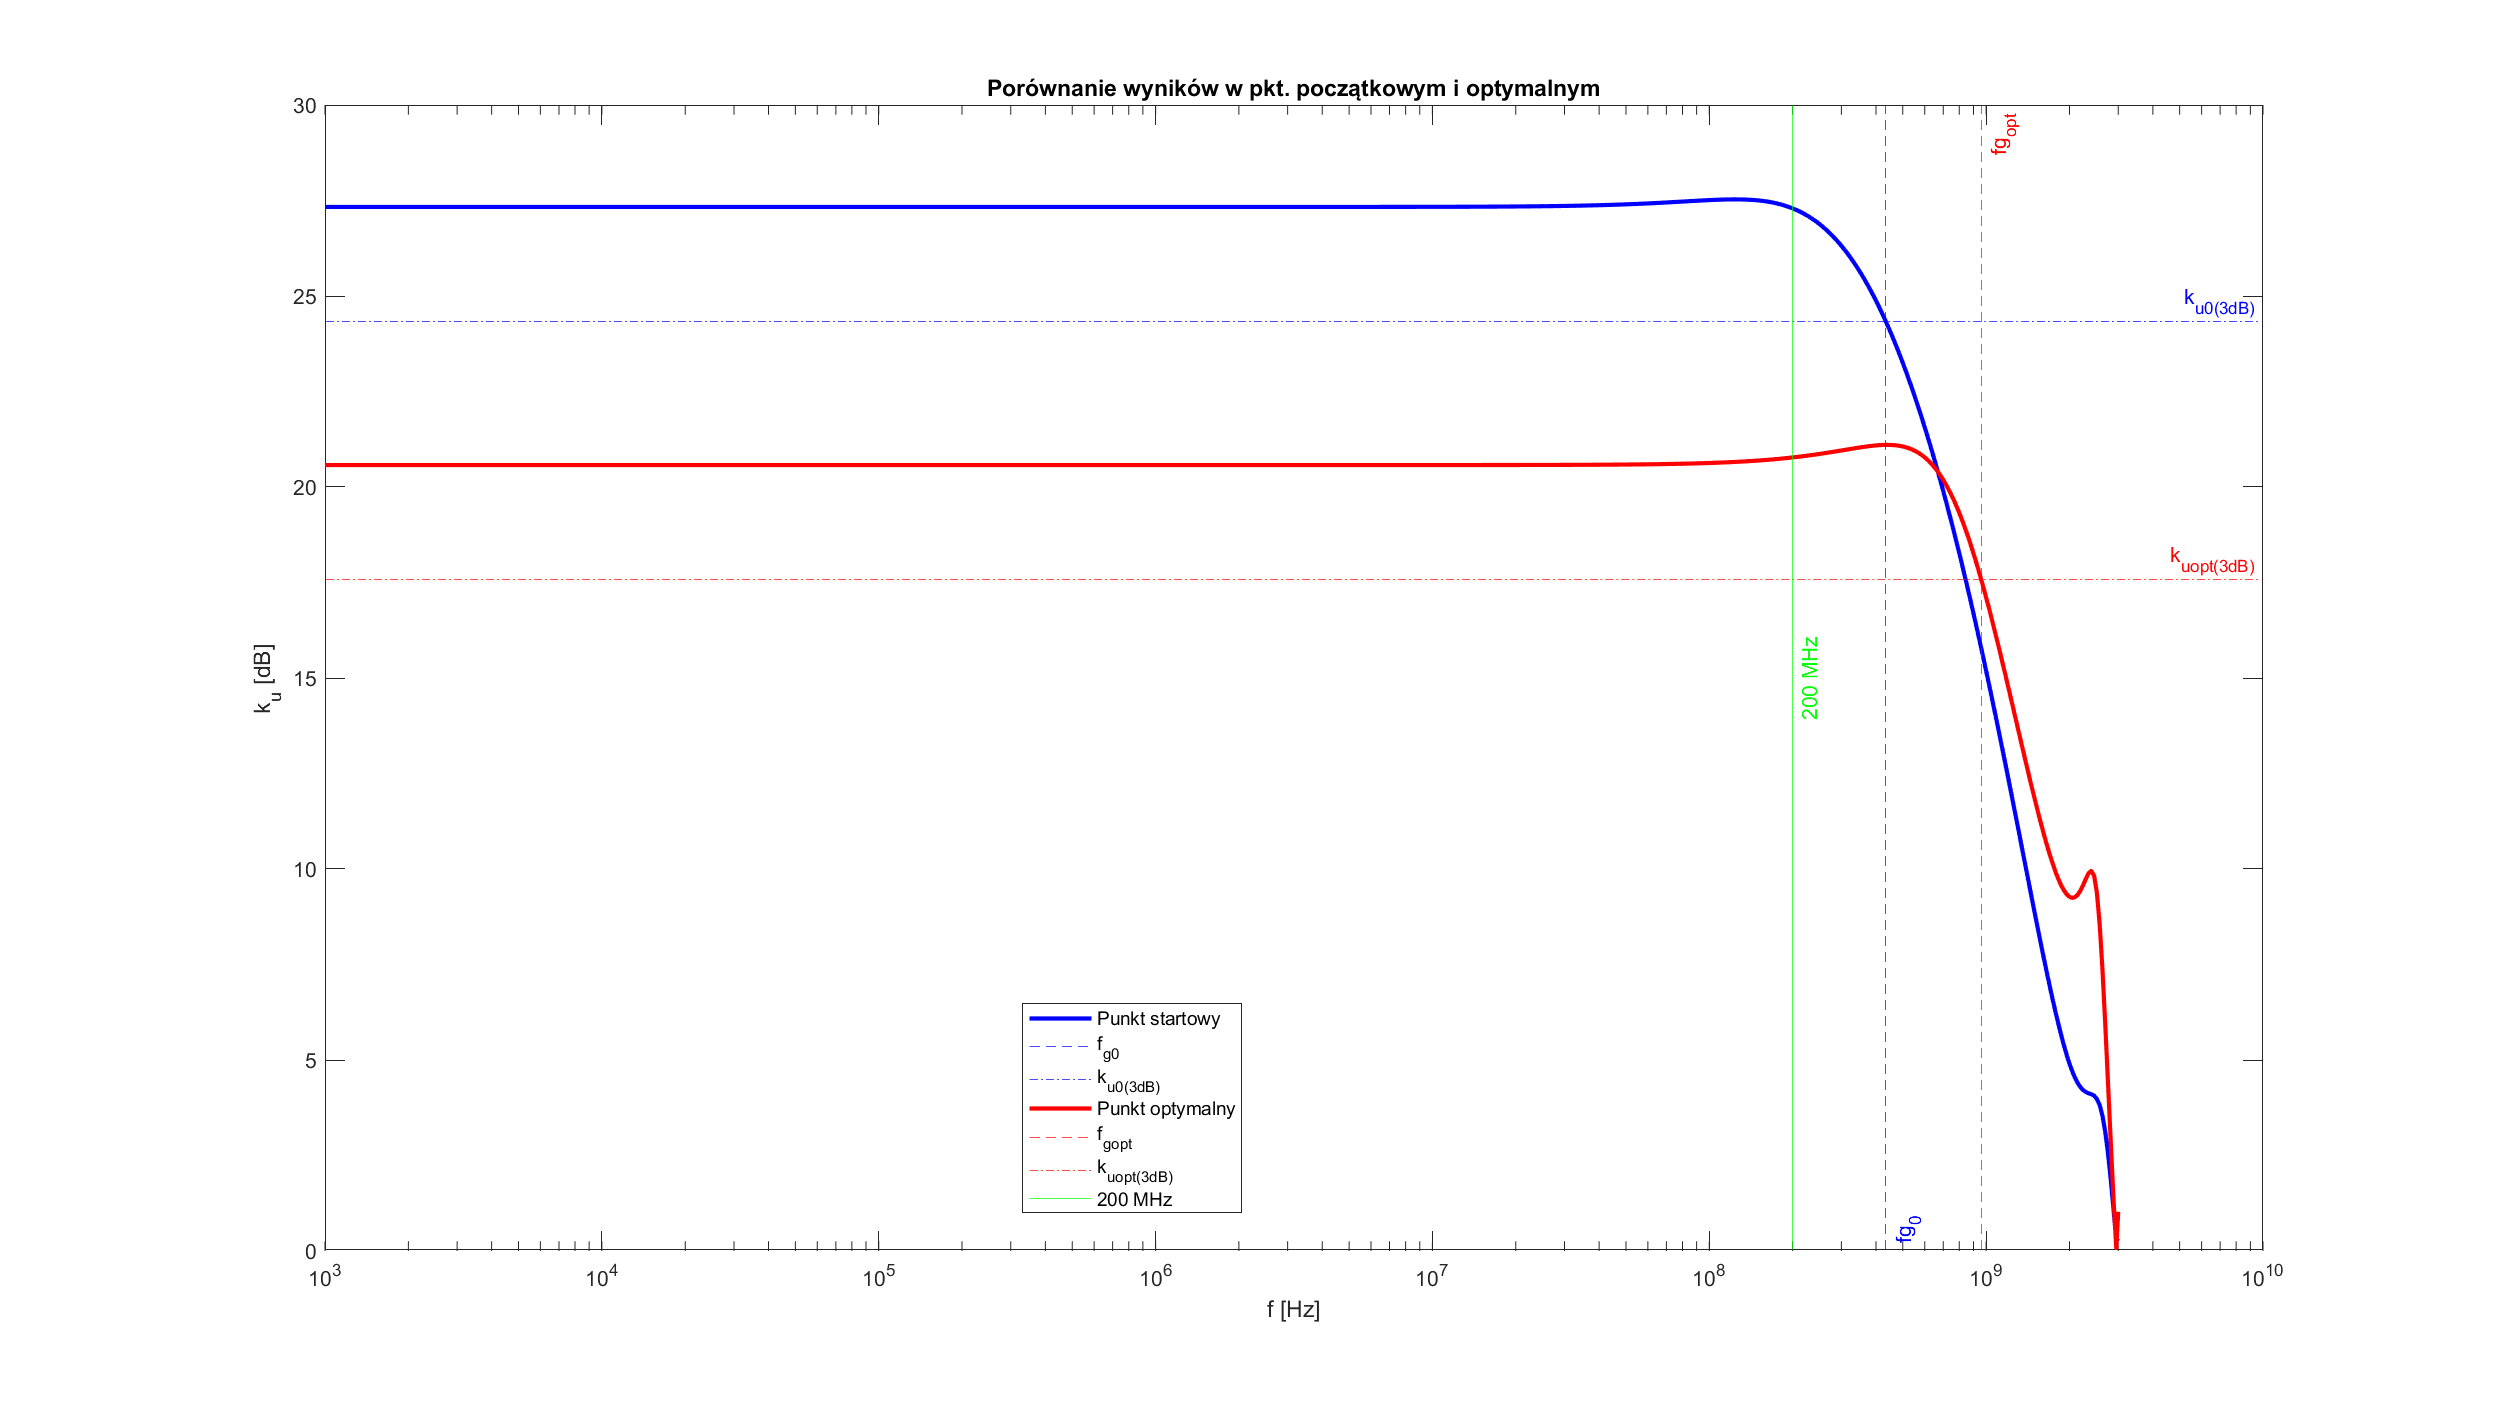
\includegraphics[width=12cm]{graphics/comparison.png}
% 	\centering
% 	\caption{Porównanie punktu optymalnego i startowego.}
% \end{figure}

% \begin{figure}[h]
% 	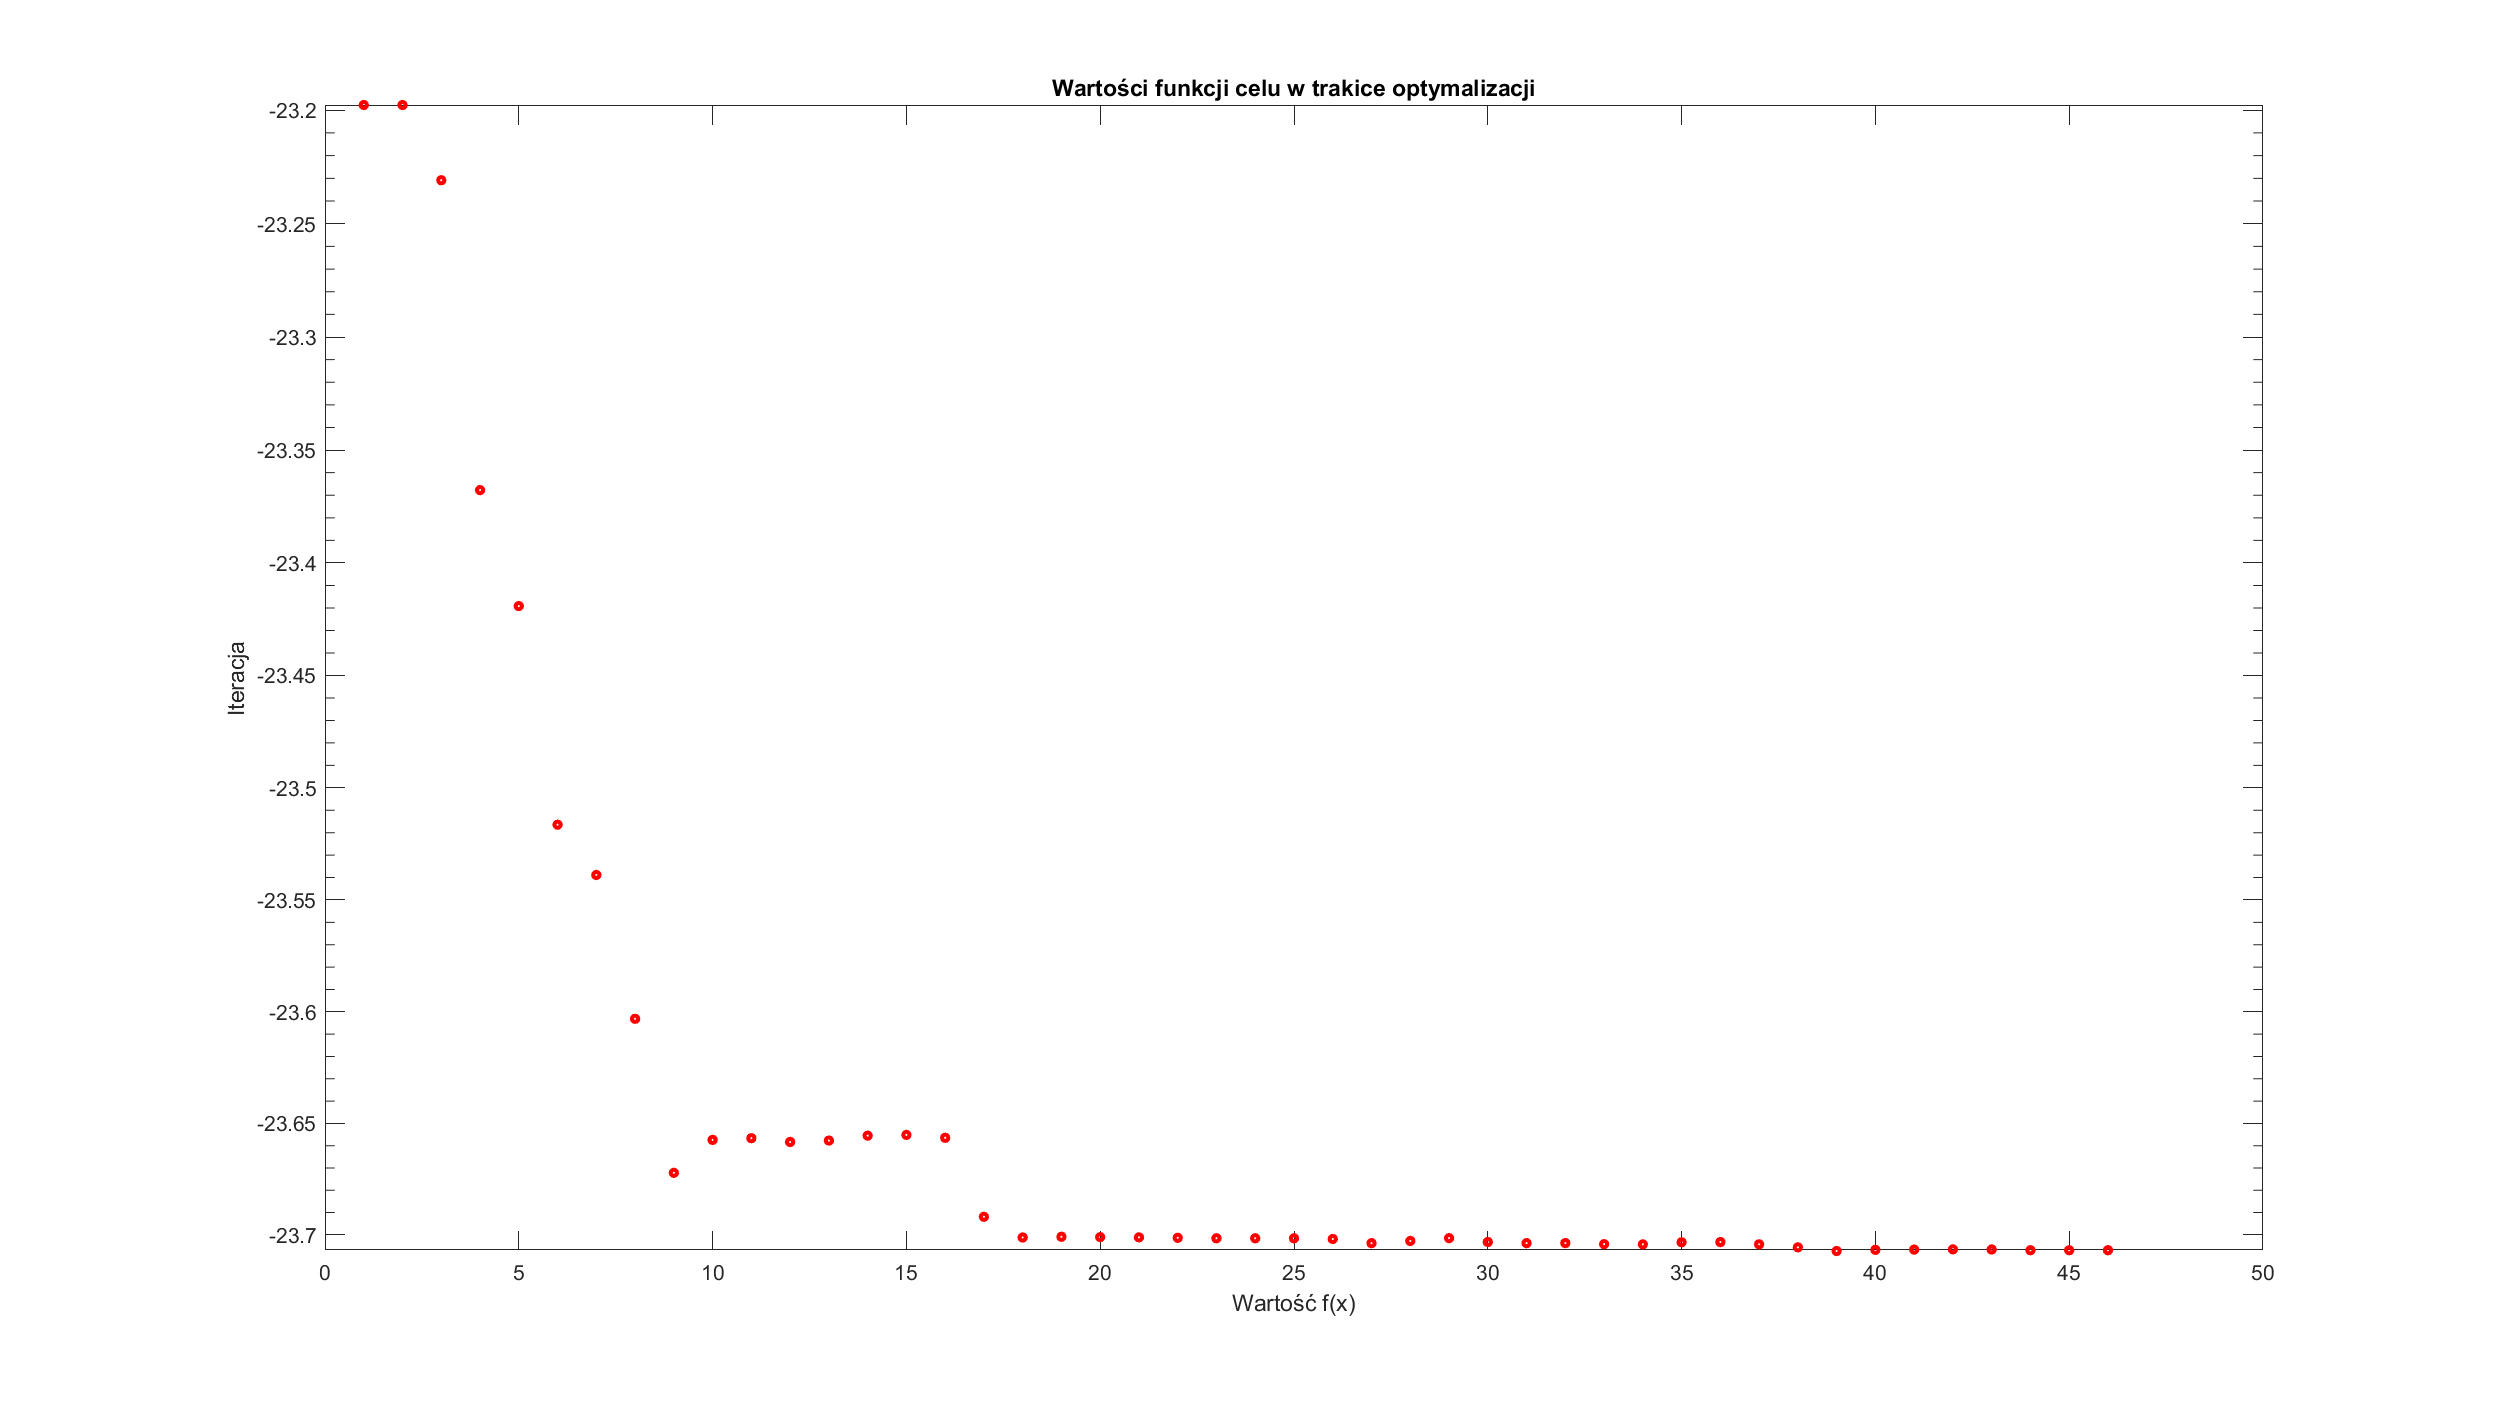
\includegraphics[width=12cm]{graphics/fval.png}
% 	\centering
% 	\caption{Przebieg wartości funkcji celu.}
% \end{figure}

% \begin{figure}[h]
% 	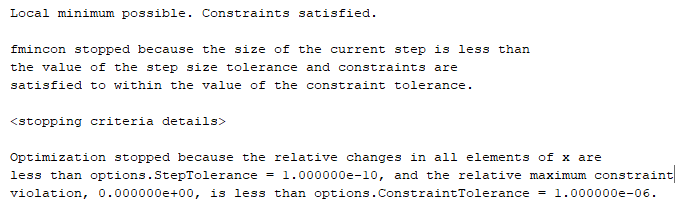
\includegraphics[width=10cm]{graphics/exit_msg.png}
% 	\centering
% 	\caption{Informacja o zakończeniu pracy przez optymalizator.}
% \end{figure}


% \begin{figure}[h]
% 	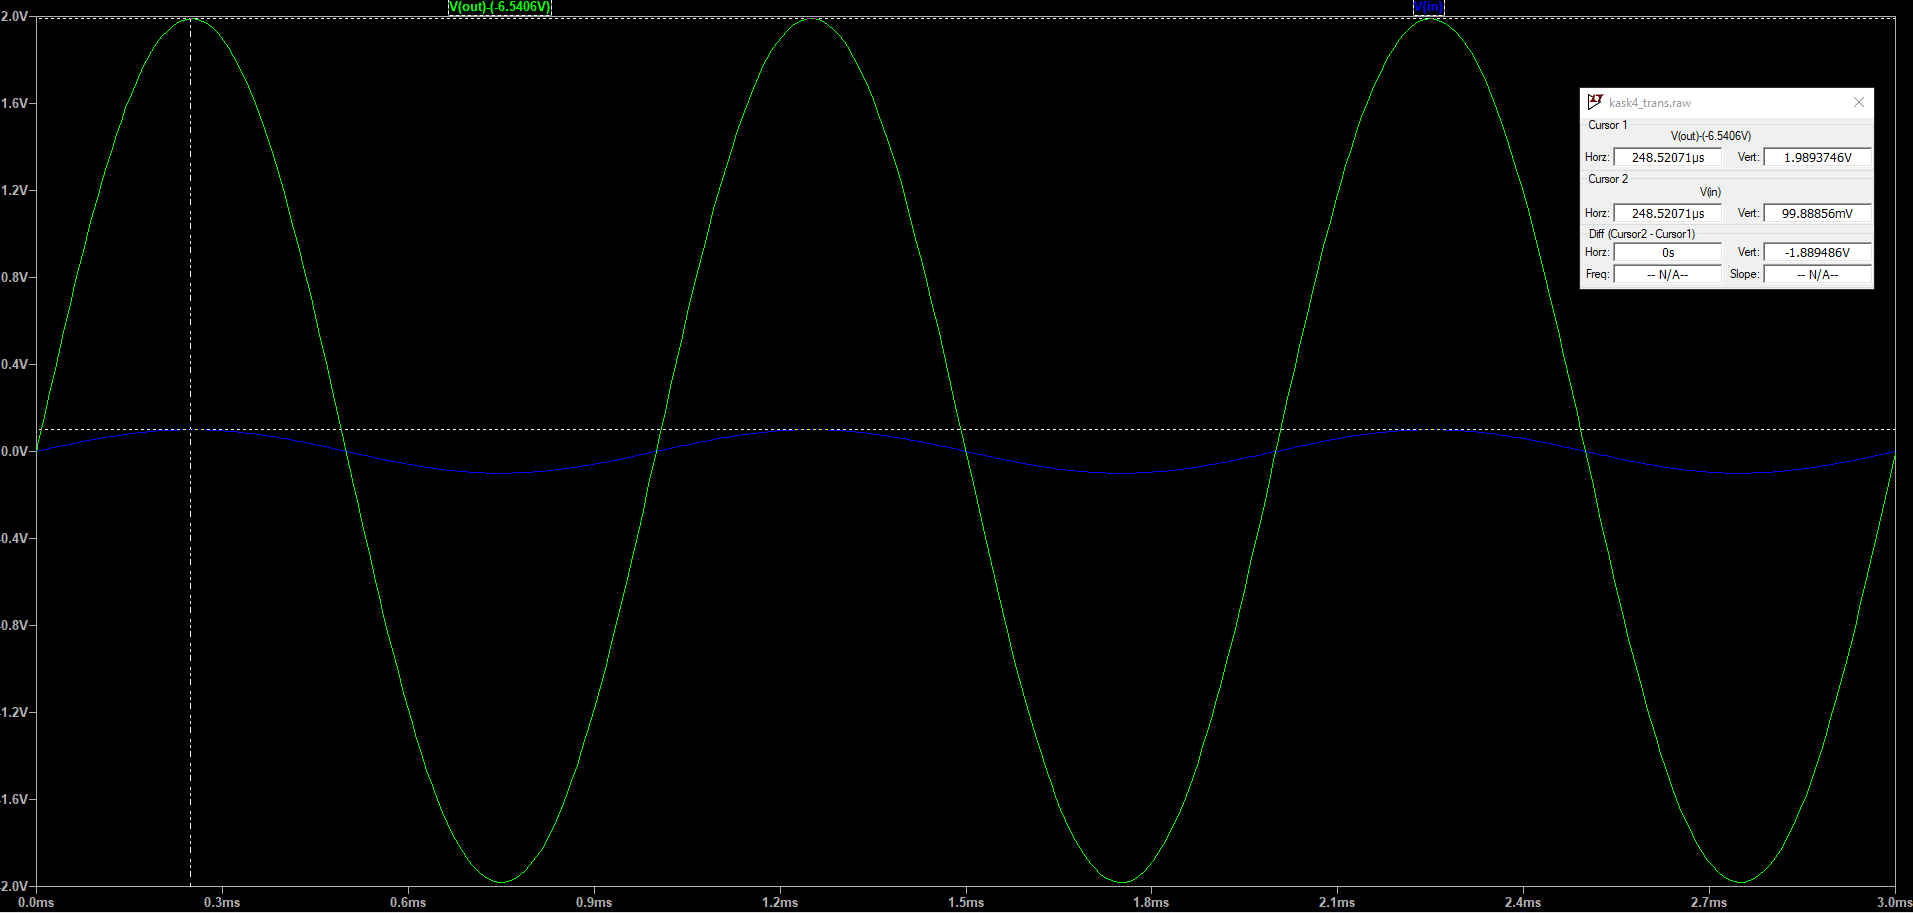
\includegraphics[width=10cm,height=4cm]{graphics/optim_tran.png}
% 	\centering
% 	\caption{Symulacja czasowa w pkt. optymalnym. Wzmacniacz wzmacnia.}
% \end{figure}


\pagebreak









\clearpage
\section{Grafiki w wysokiej rozdzielczości.}


\begin{landscape}
	\begin{figure}[h]
		\vspace*{-2cm}
		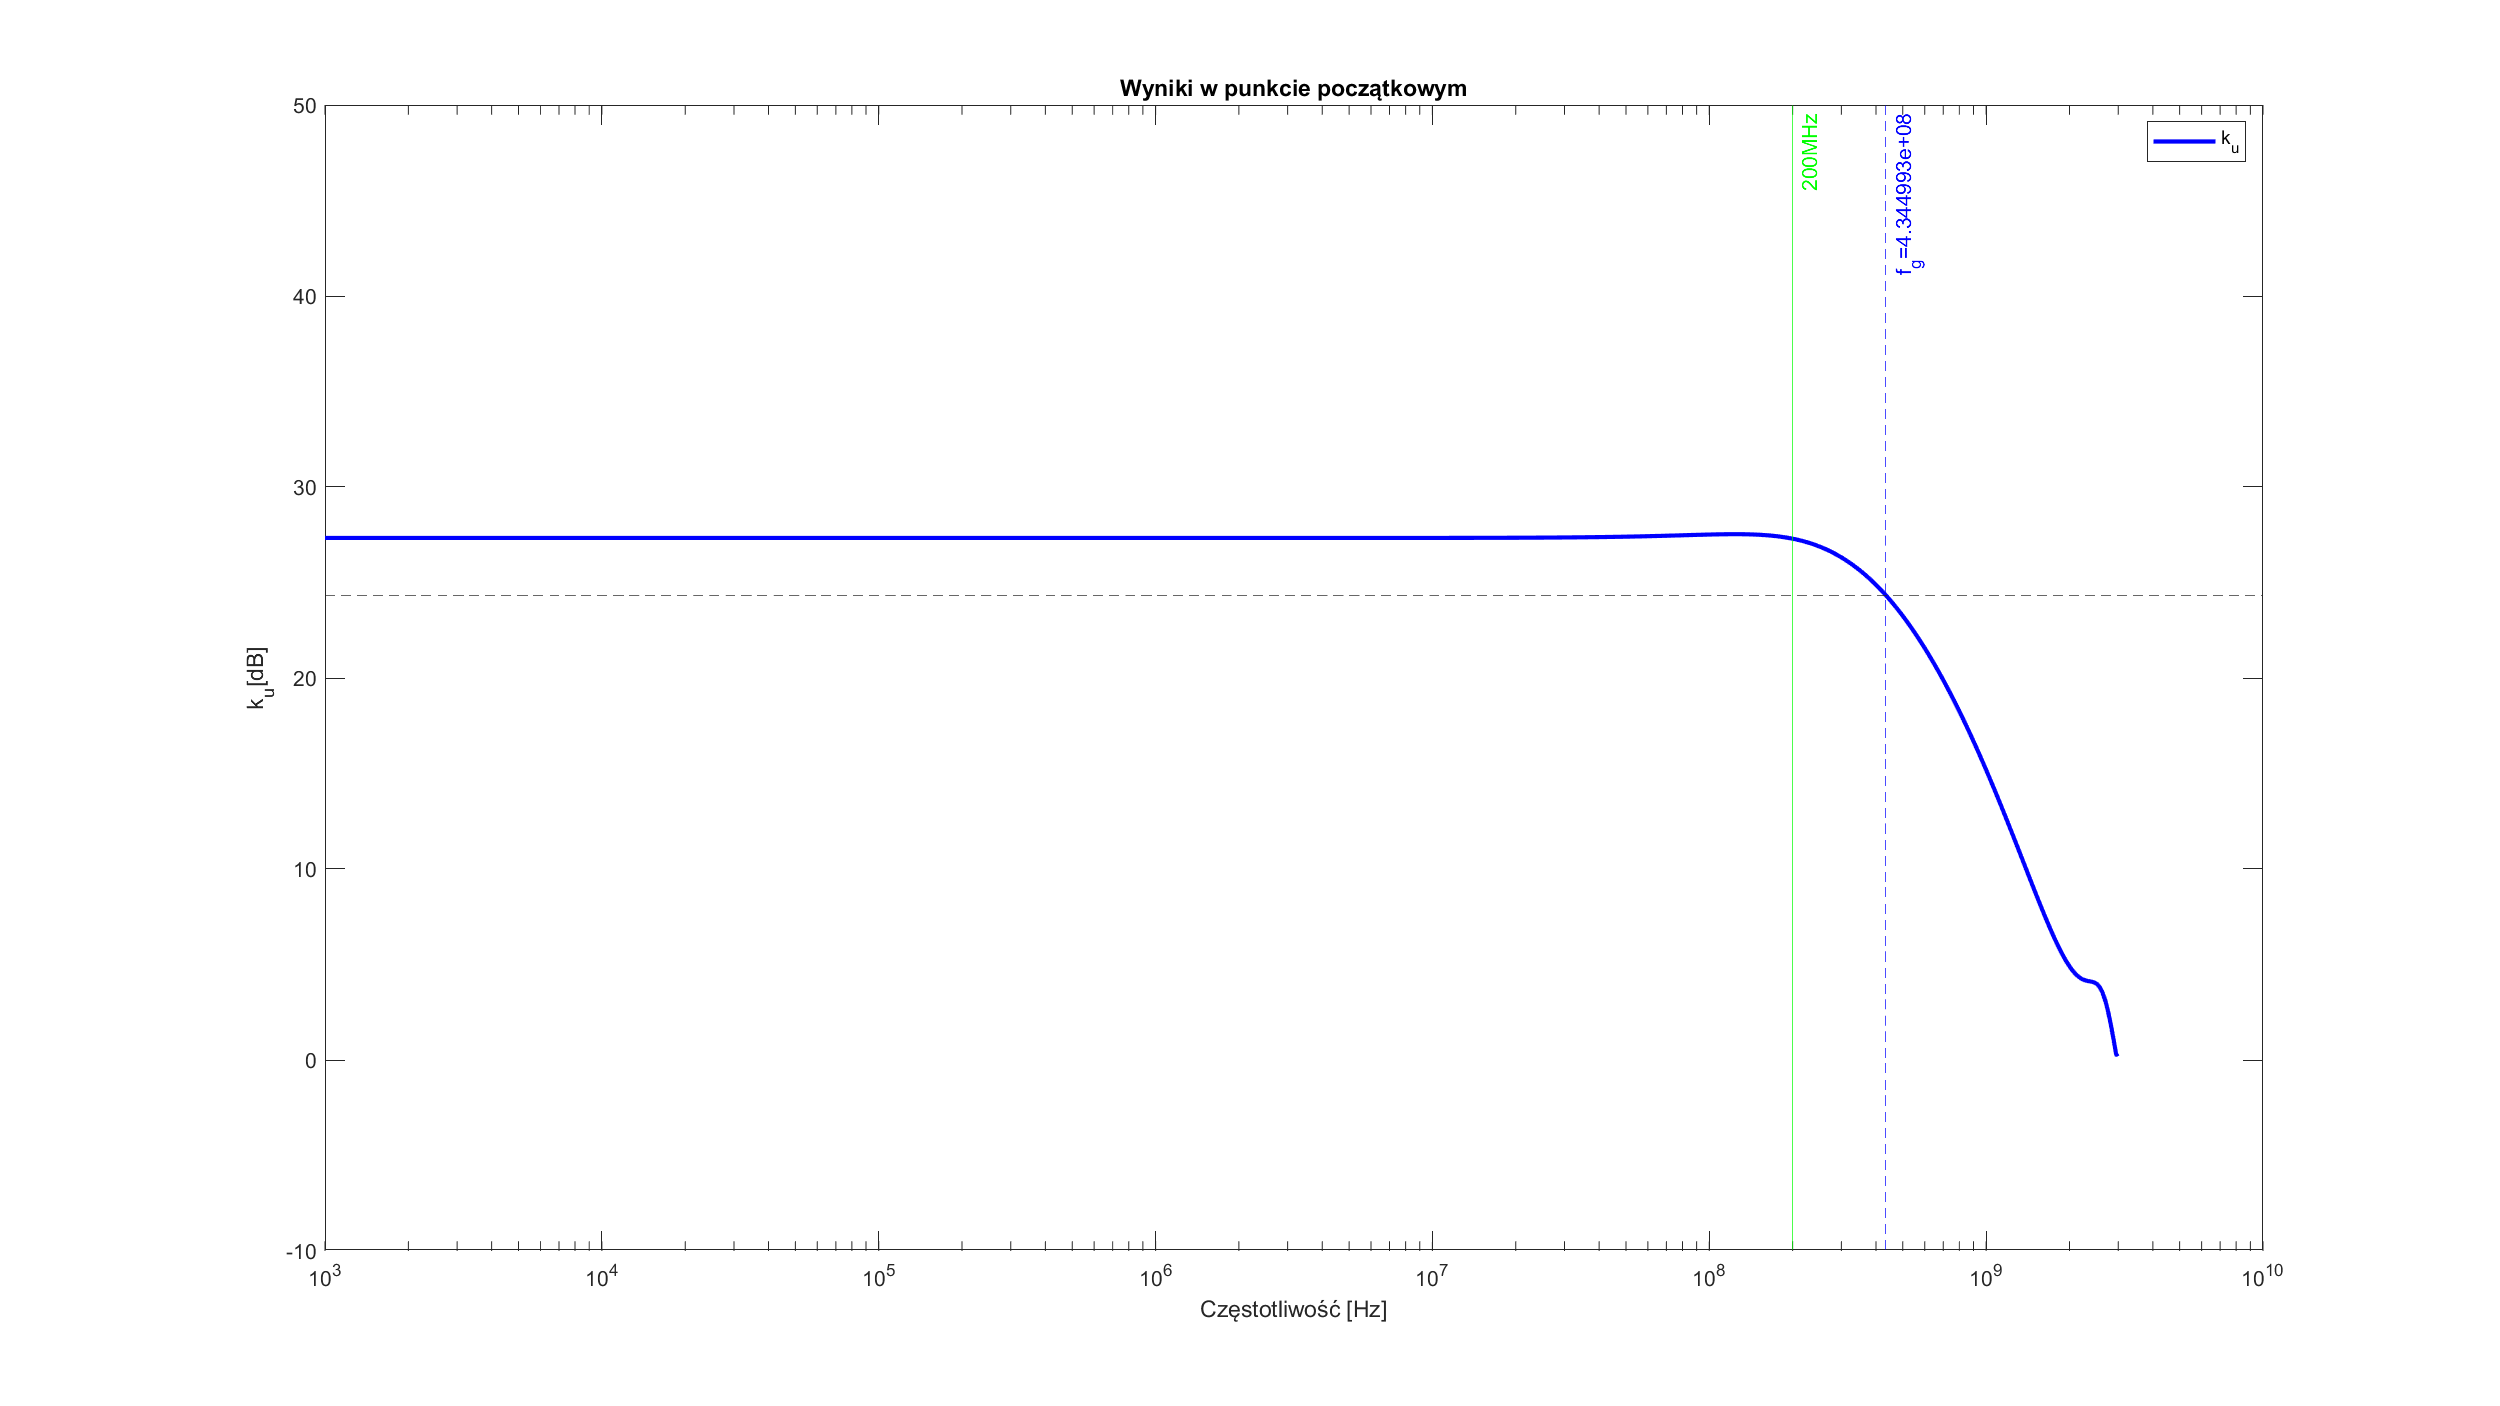
\includegraphics[width=25cm,height=15 cm]{graphics/starting_point.png}
		\centering
		\caption{Charakterystyka układu w punkcie startowym.}
	\end{figure}
\end{landscape}

\clearpage
\pagebreak
\begin{landscape}
	\begin{figure}[h]
		\vspace*{-2cm}
		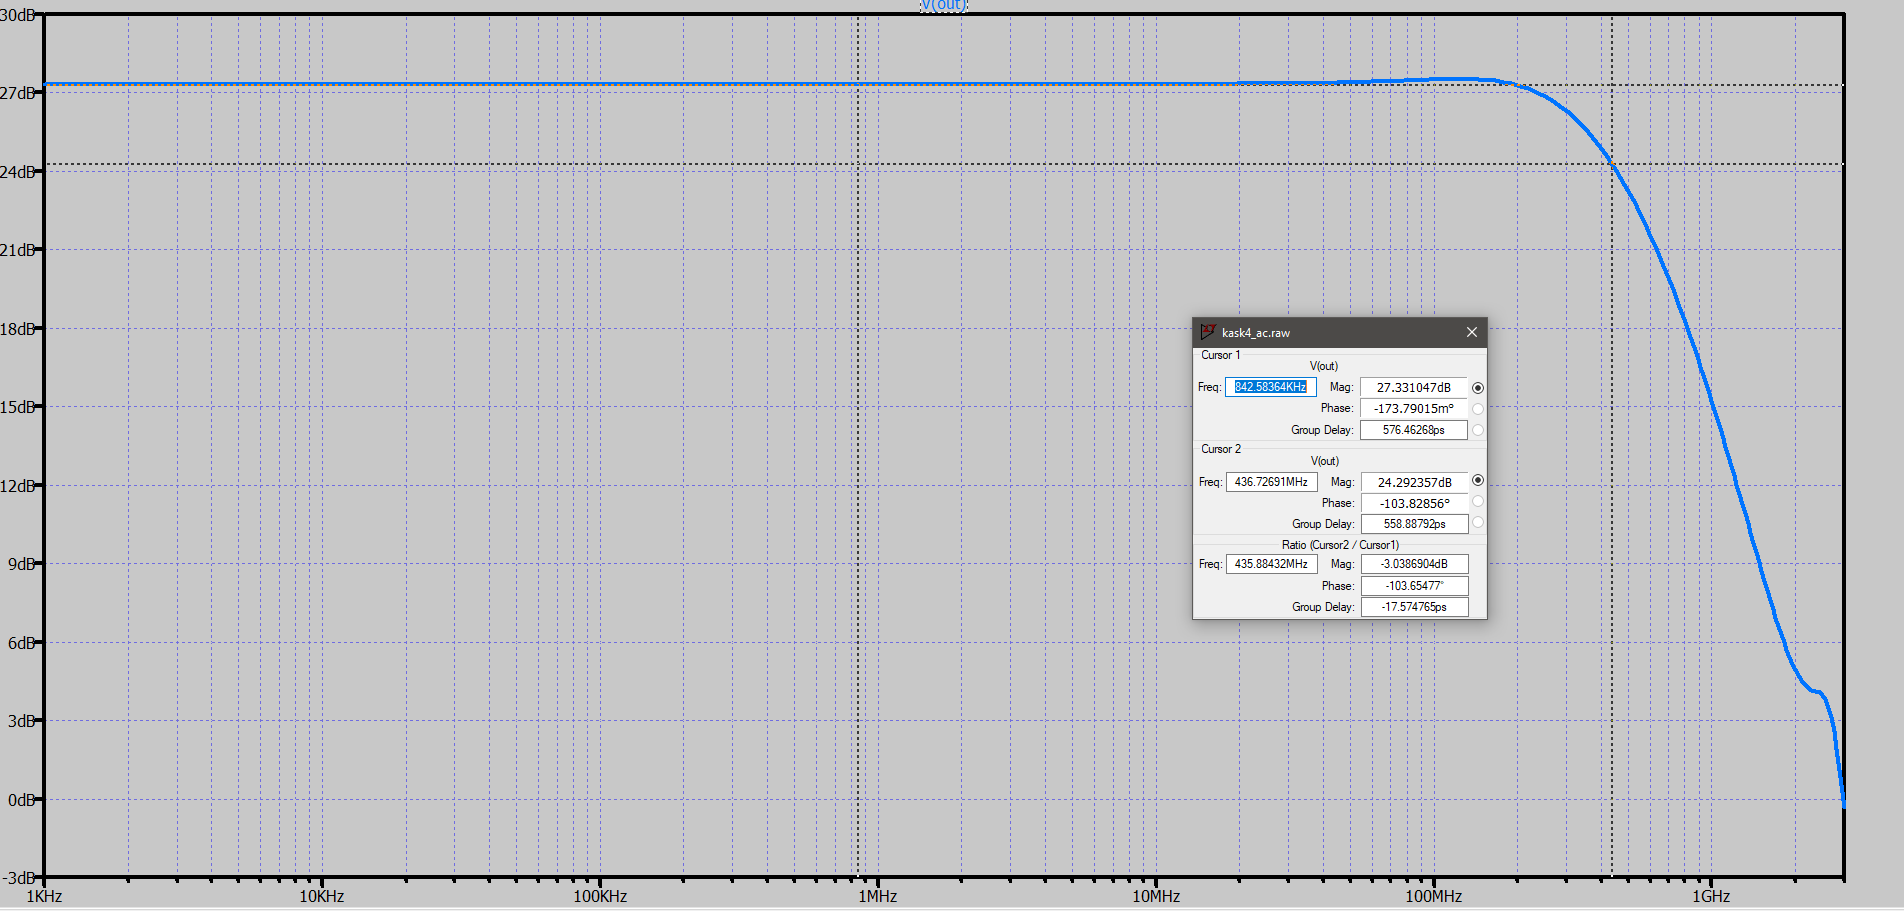
\includegraphics[width=20cm,height=10 cm]{graphics/starting_point_spice.png}
		\centering
		\caption{Charakterystyka układu w punkcie startowym (LTSpice).}
	\end{figure}
\end{landscape}

\pagebreak
\begin{landscape}
	\begin{figure}[h]
		\vspace*{-2cm}
		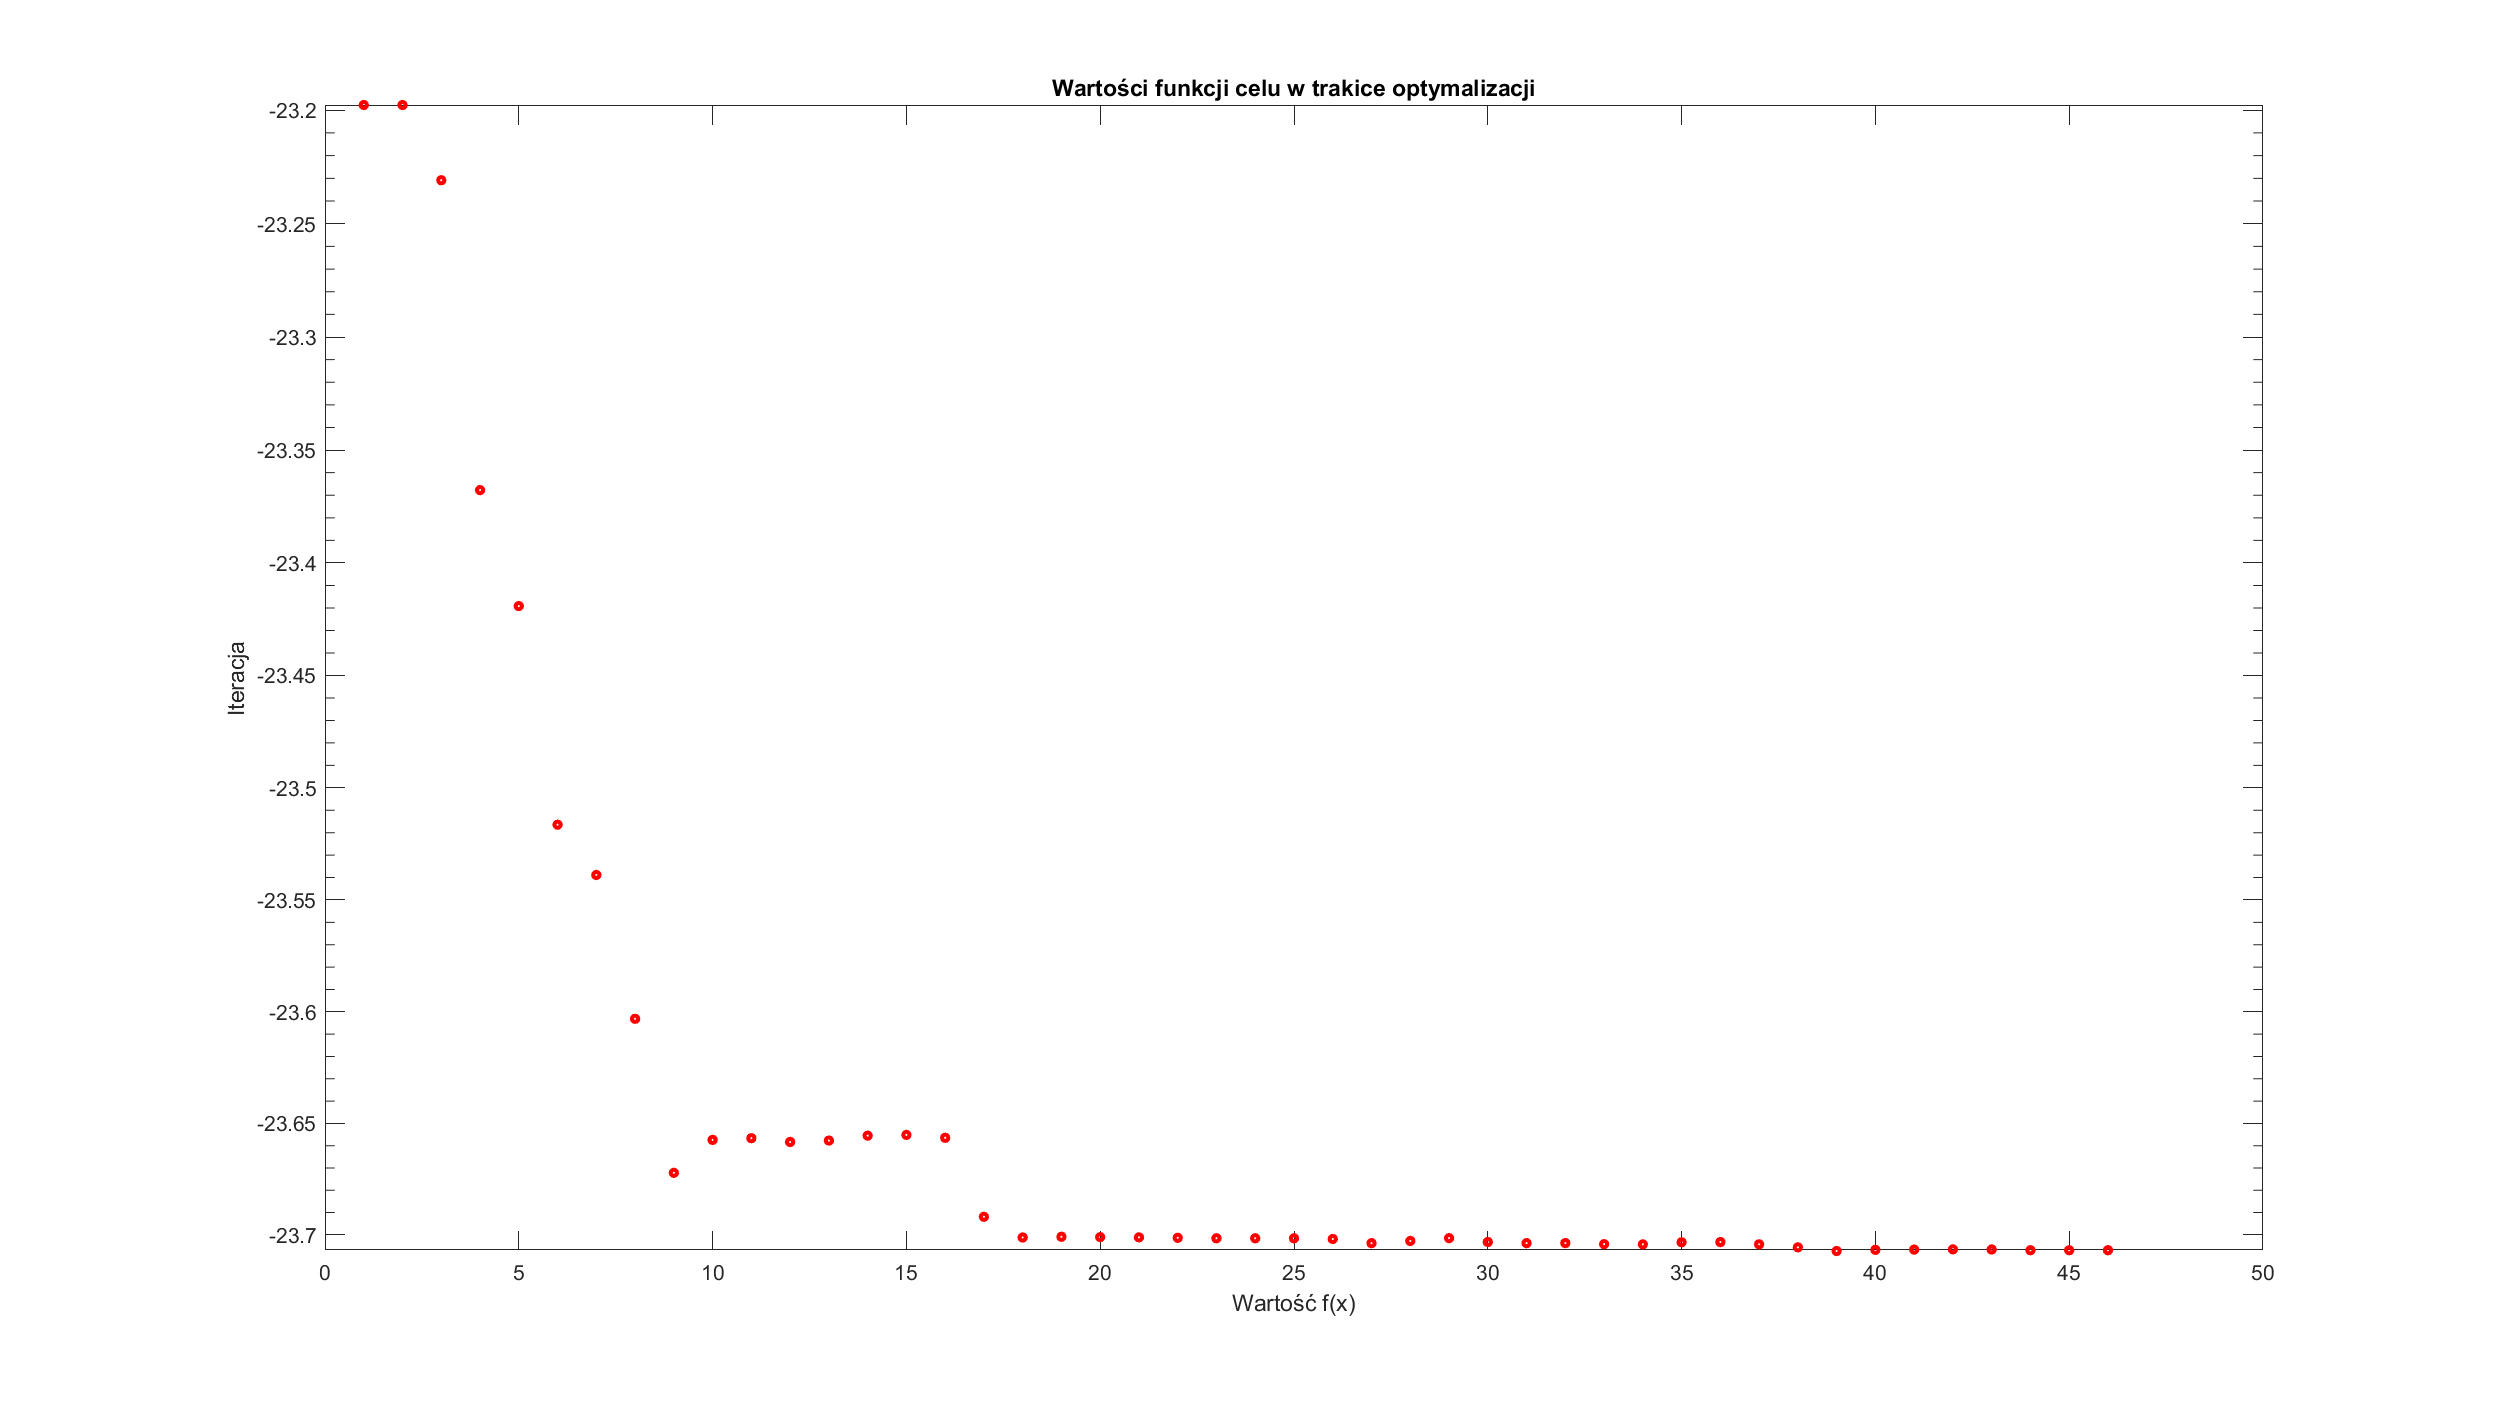
\includegraphics[width=25cm,height=15 cm]{graphics/fval.png}
		\centering
		\caption{Przebieg wartości funkcji celu.}
	\end{figure}
\end{landscape}

\pagebreak
\begin{landscape}
	\begin{figure}[h]
		\vspace*{-2cm}
		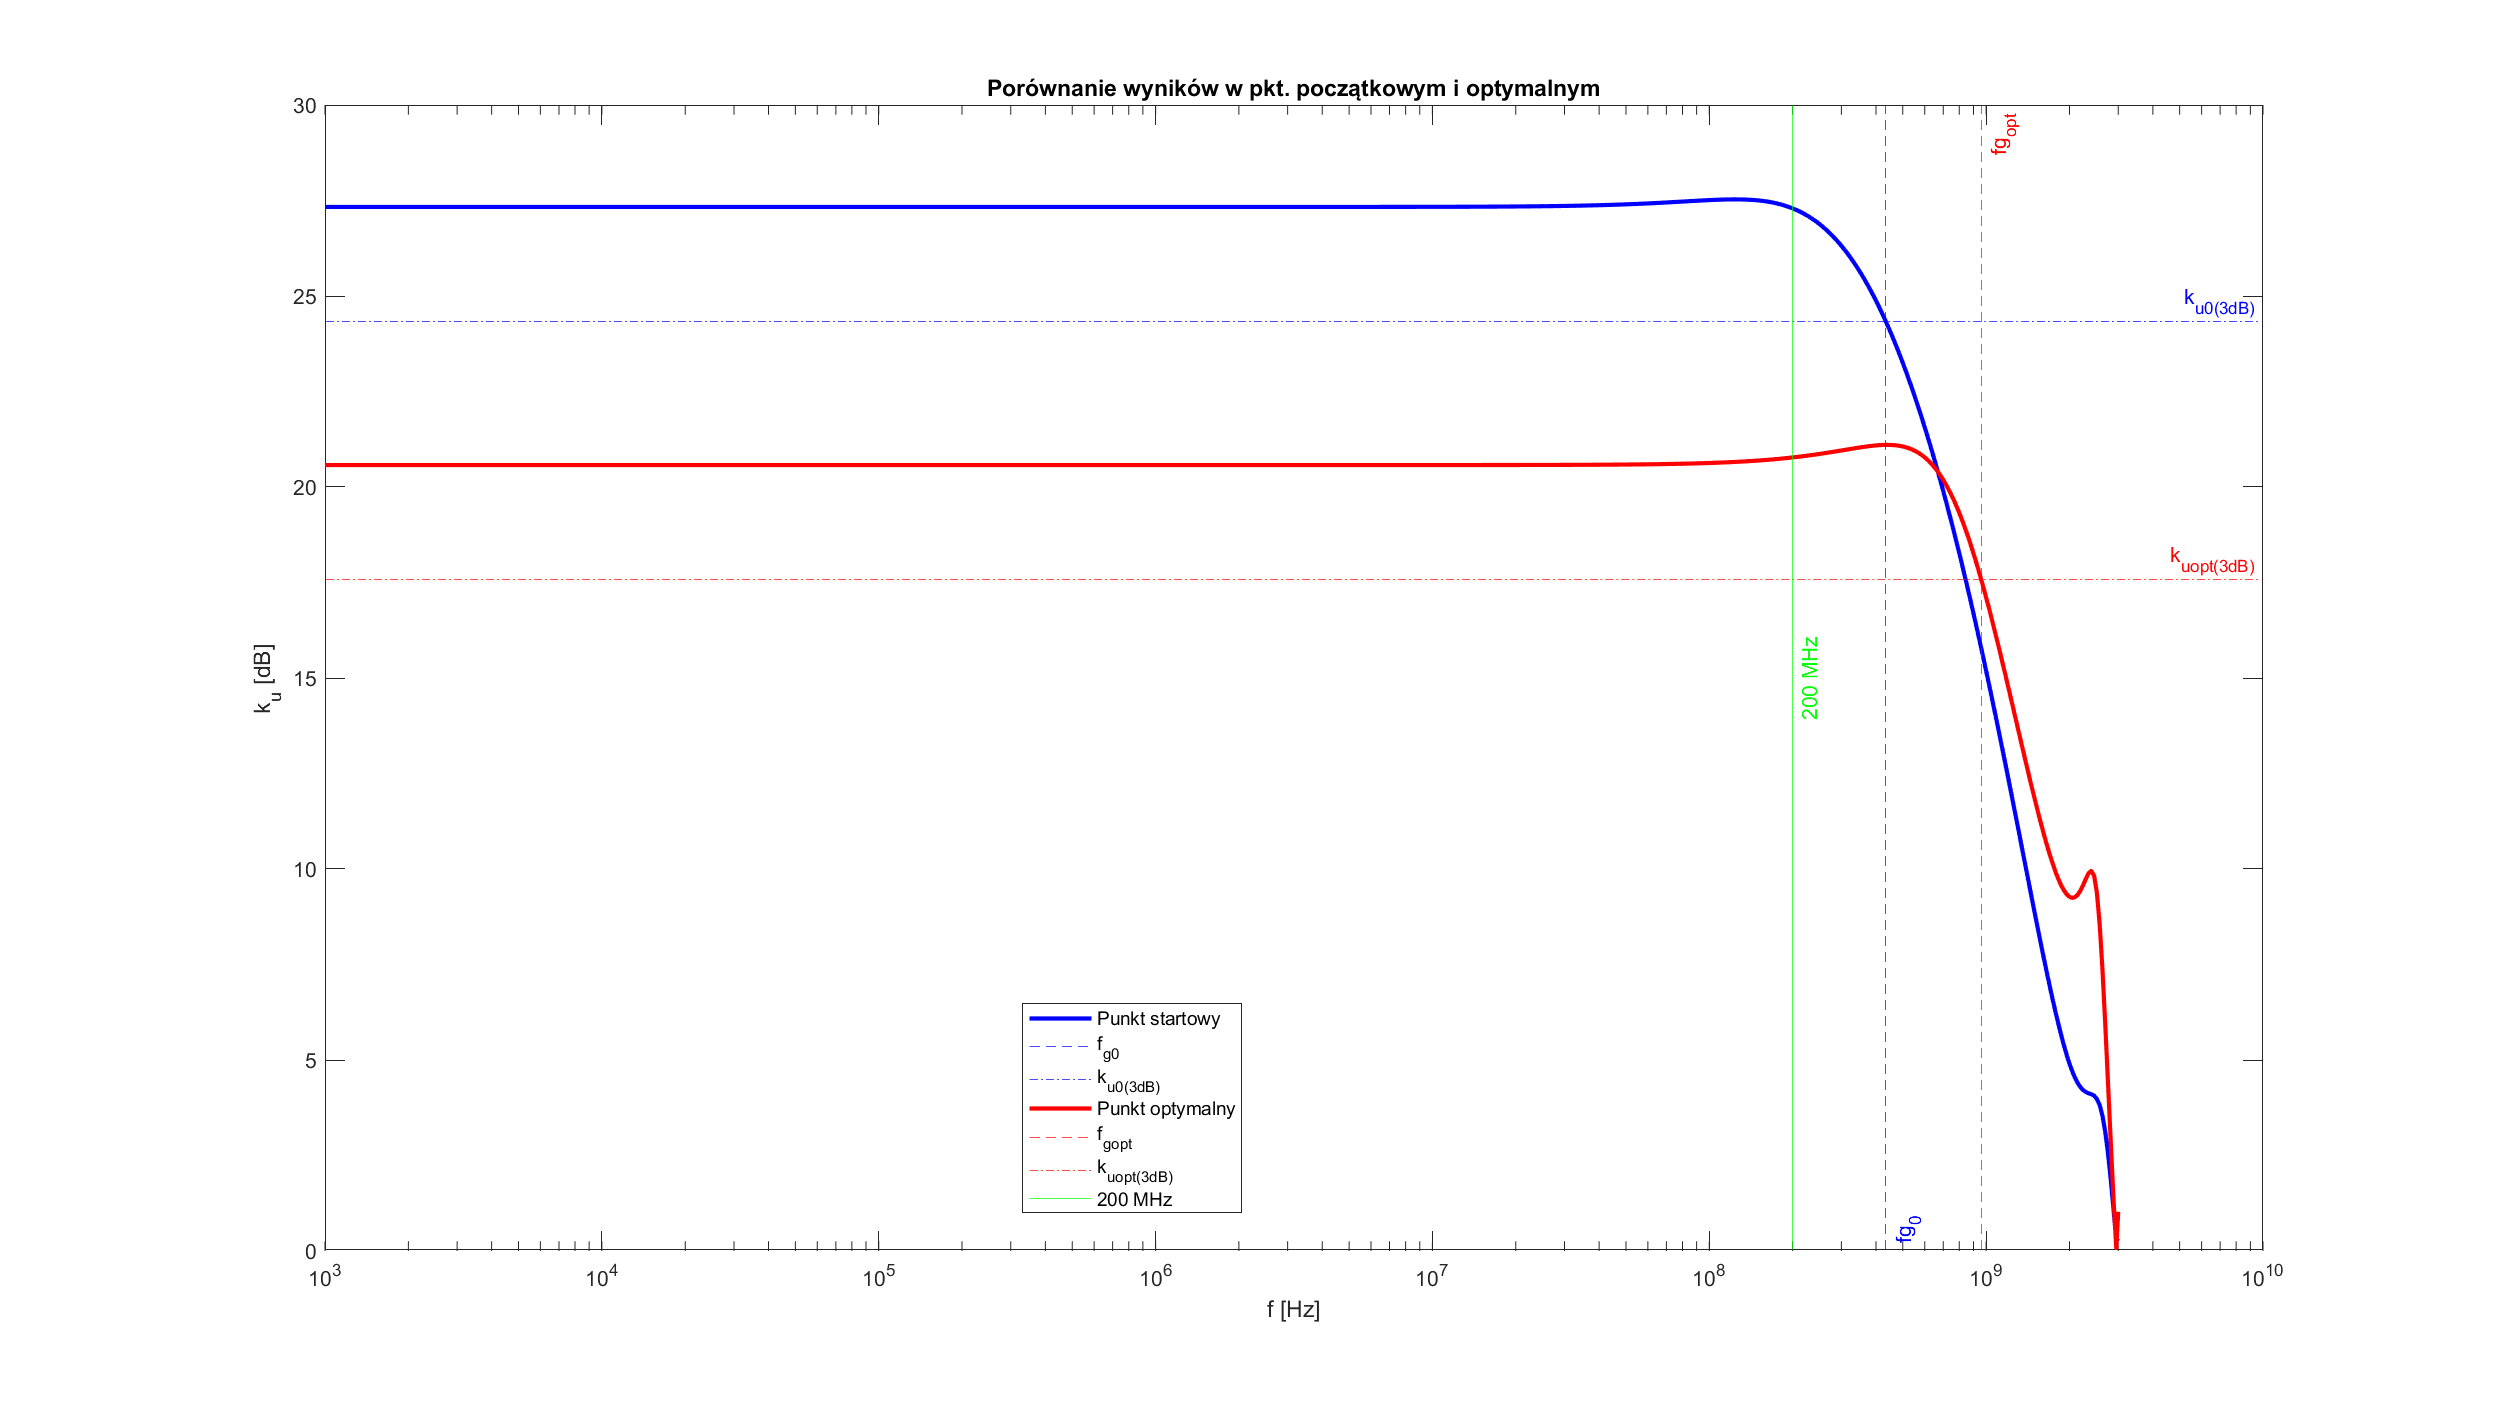
\includegraphics[width=25cm,height=15 cm]{graphics/comparison.png}
		\centering
		\caption{Porównanie wyników w punkcie optymalnym i startowym.}
	\end{figure}
\end{landscape}


\pagebreak
\begin{landscape}
	\begin{figure}[h]
		\vspace*{-2cm}
		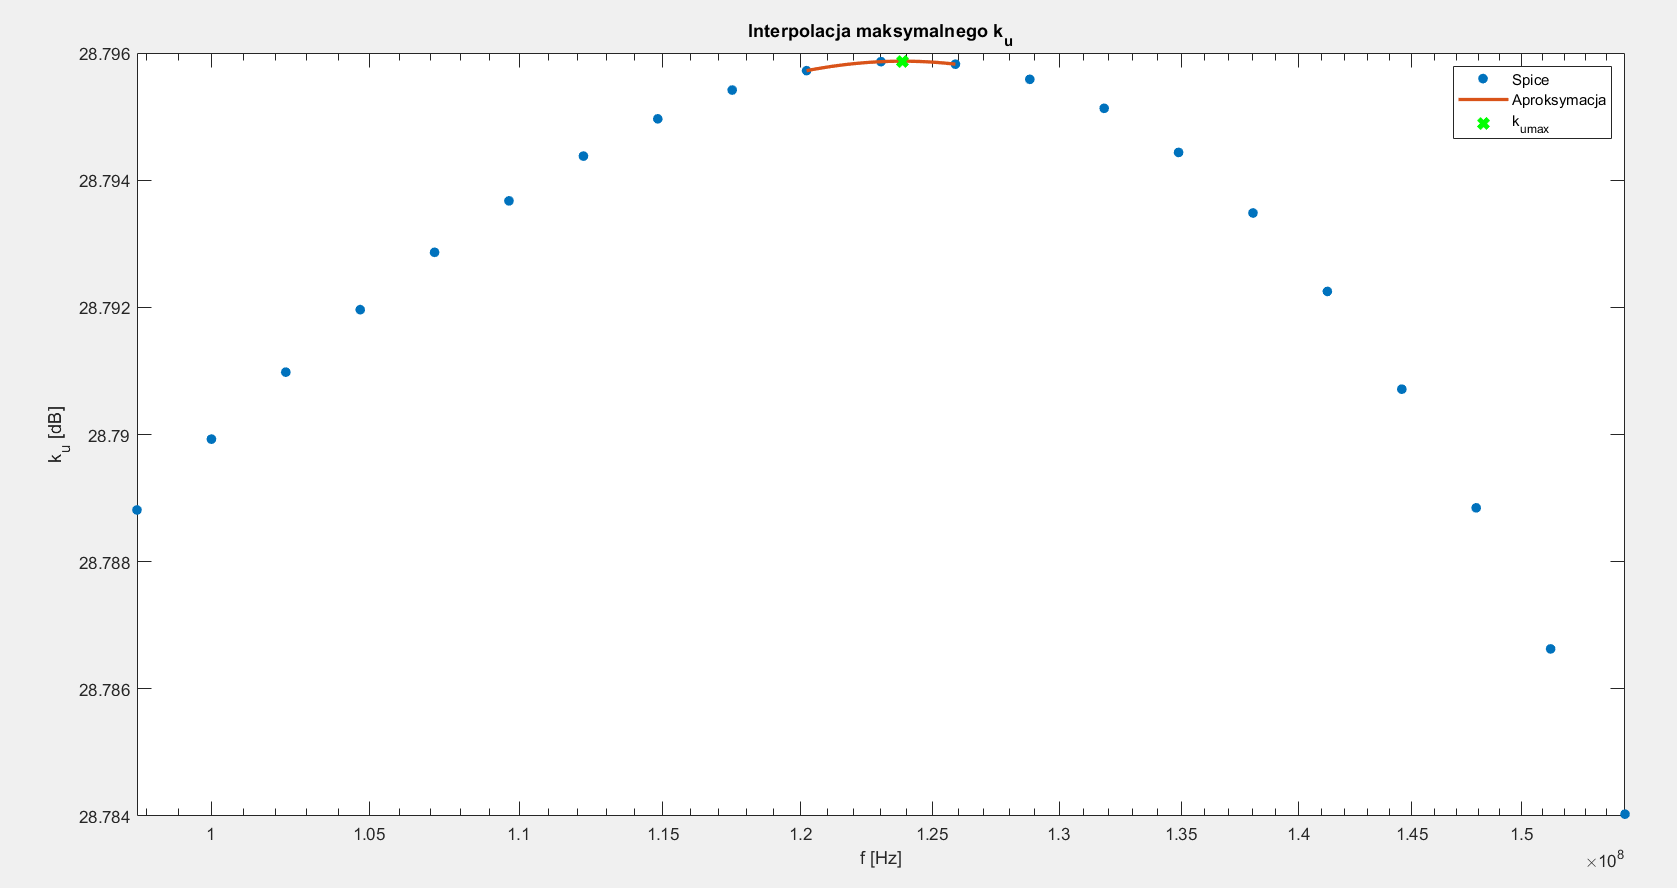
\includegraphics[width=20cm,height=10 cm]{graphics/max_ku_interp.png}
		\centering
		\caption{Interpolacja maksymalnego wzmocnienia.}
	\end{figure}
\end{landscape}

\pagebreak
\begin{landscape}
	\begin{figure}[h]
		\vspace*{-2cm}
		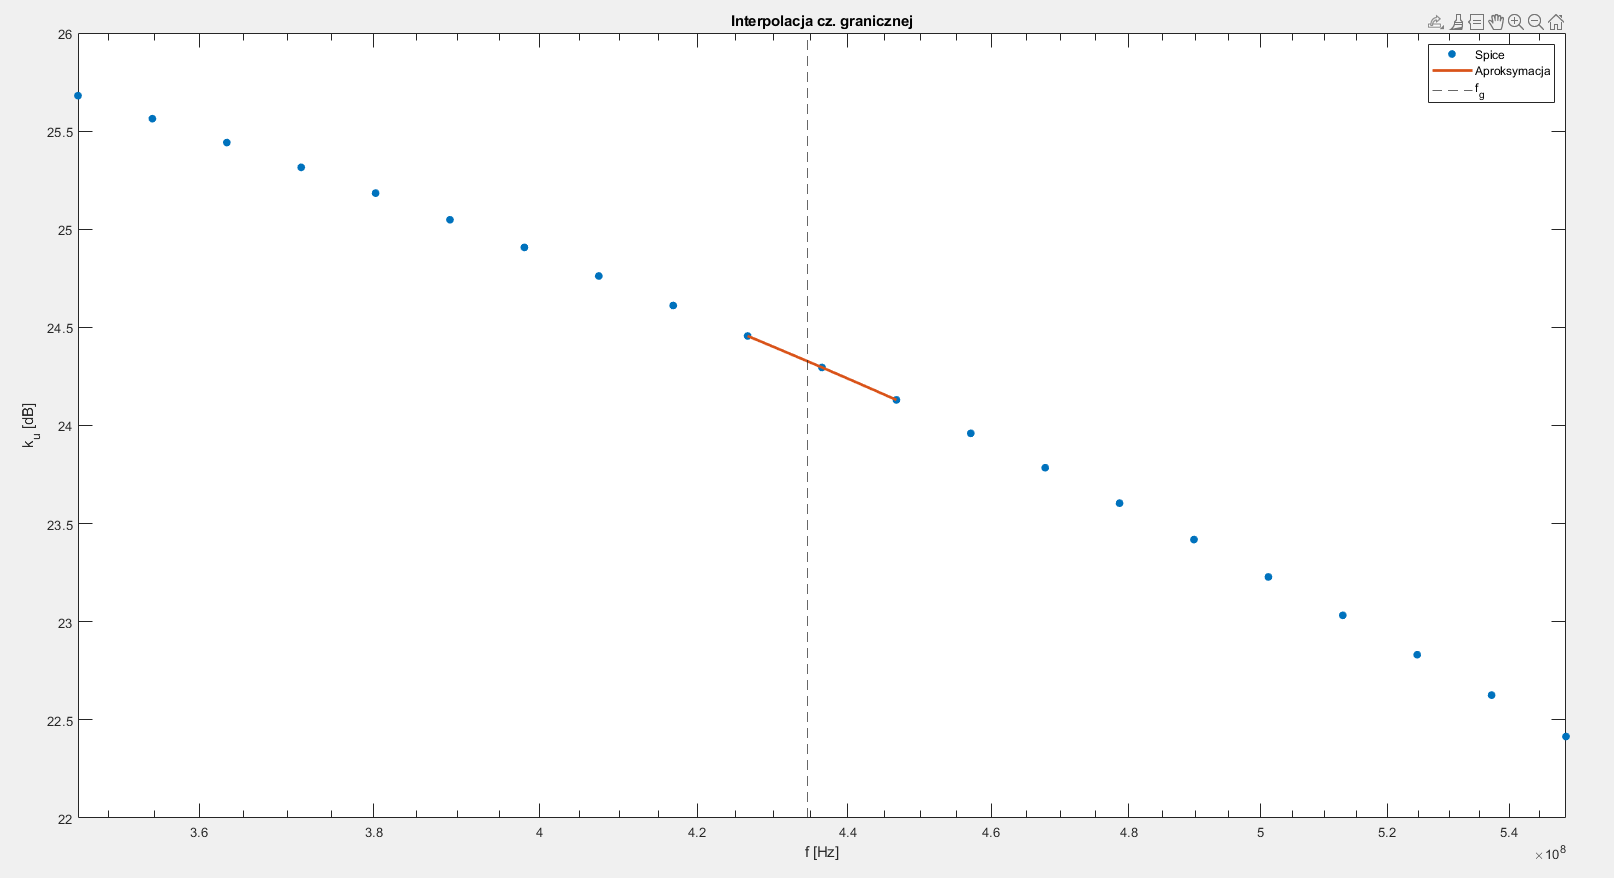
\includegraphics[width=20cm,height=10 cm]{graphics/fg_interp.png}
		\centering
		\caption{Interpolacja częstotliwości granicznej.}
	\end{figure}
\end{landscape}

\pagebreak
\begin{landscape}
	\begin{figure}[h]
		\vspace*{-2cm}
		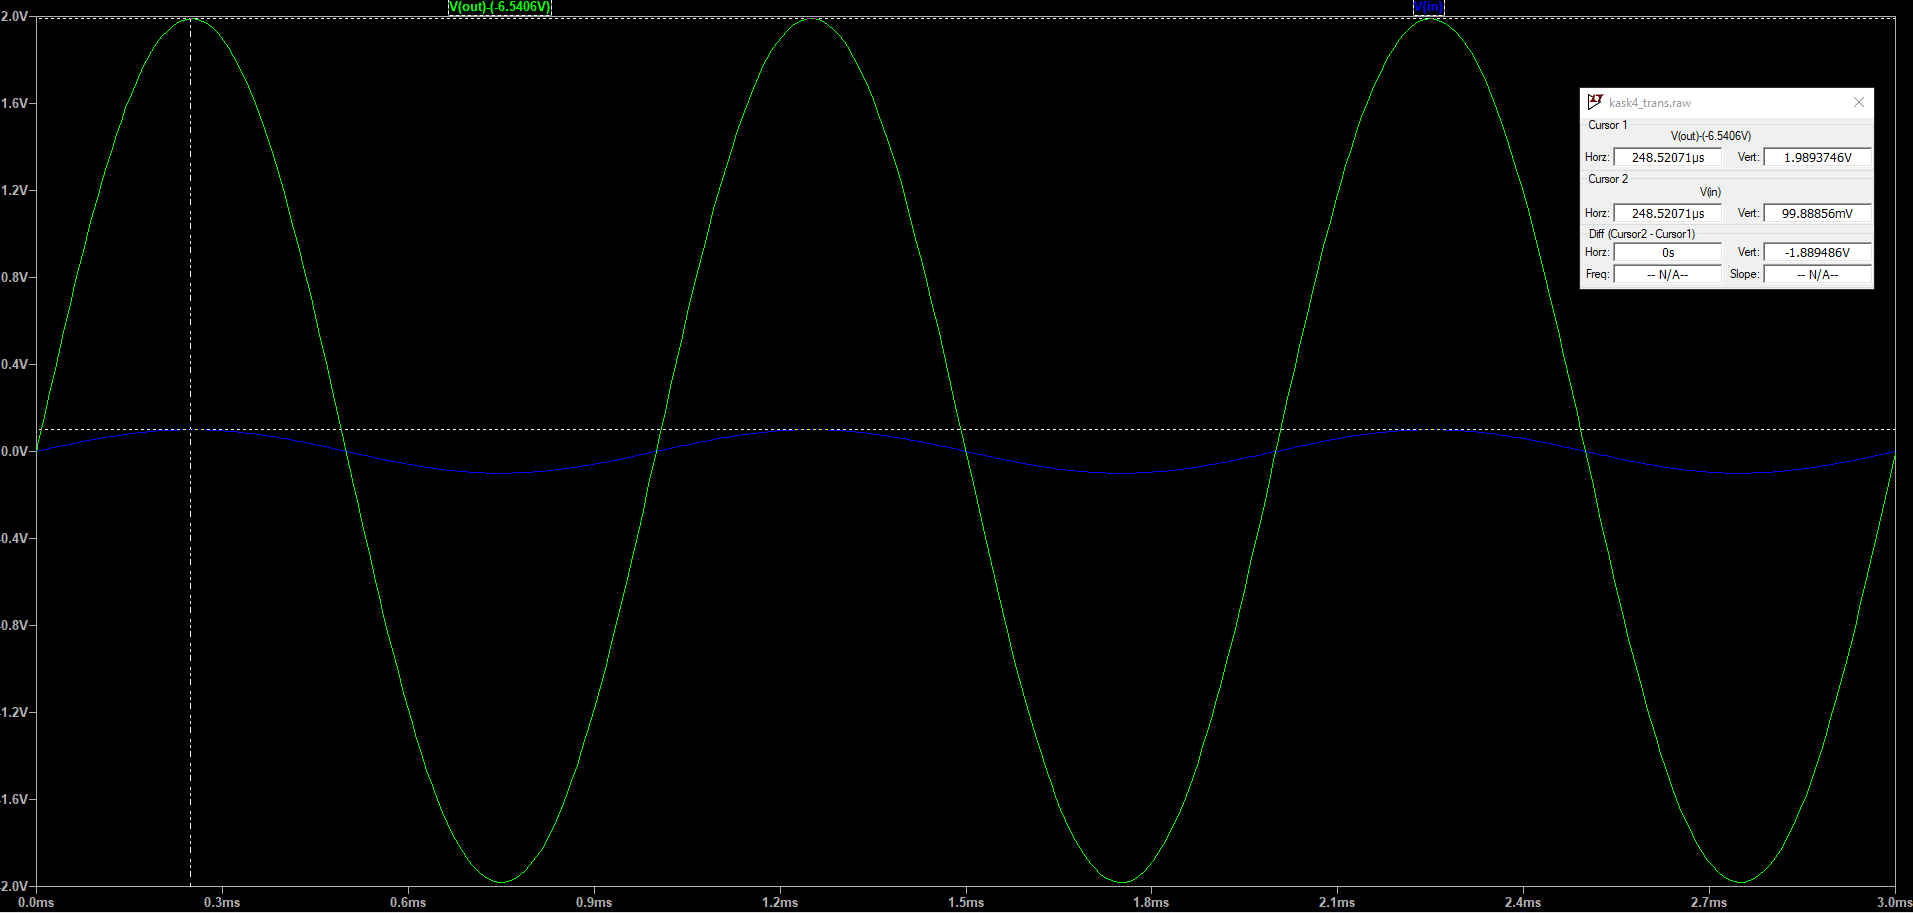
\includegraphics[width=20cm,height=10cm]{graphics/optim_tran.png}
		\centering
		\caption{Symulacja czasowa w pkt. optymalnym. Wzmacniacz wzmacnia.}
	\end{figure}
\end{landscape}

\end{document}


